% Options for packages loaded elsewhere
\PassOptionsToPackage{unicode}{hyperref}
\PassOptionsToPackage{hyphens}{url}
%
\documentclass[
]{book}
\usepackage{amsmath,amssymb}
\usepackage{lmodern}
\usepackage{iftex}
\ifPDFTeX
  \usepackage[T1]{fontenc}
  \usepackage[utf8]{inputenc}
  \usepackage{textcomp} % provide euro and other symbols
\else % if luatex or xetex
  \usepackage{unicode-math}
  \defaultfontfeatures{Scale=MatchLowercase}
  \defaultfontfeatures[\rmfamily]{Ligatures=TeX,Scale=1}
\fi
% Use upquote if available, for straight quotes in verbatim environments
\IfFileExists{upquote.sty}{\usepackage{upquote}}{}
\IfFileExists{microtype.sty}{% use microtype if available
  \usepackage[]{microtype}
  \UseMicrotypeSet[protrusion]{basicmath} % disable protrusion for tt fonts
}{}
\makeatletter
\@ifundefined{KOMAClassName}{% if non-KOMA class
  \IfFileExists{parskip.sty}{%
    \usepackage{parskip}
  }{% else
    \setlength{\parindent}{0pt}
    \setlength{\parskip}{6pt plus 2pt minus 1pt}}
}{% if KOMA class
  \KOMAoptions{parskip=half}}
\makeatother
\usepackage{xcolor}
\IfFileExists{xurl.sty}{\usepackage{xurl}}{} % add URL line breaks if available
\IfFileExists{bookmark.sty}{\usepackage{bookmark}}{\usepackage{hyperref}}
\hypersetup{
  pdftitle={Graduate Fellows Handbook},
  pdfauthor={Vanessa Arias Casillas},
  hidelinks,
  pdfcreator={LaTeX via pandoc}}
\urlstyle{same} % disable monospaced font for URLs
\usepackage{longtable,booktabs,array}
\usepackage{calc} % for calculating minipage widths
% Correct order of tables after \paragraph or \subparagraph
\usepackage{etoolbox}
\makeatletter
\patchcmd\longtable{\par}{\if@noskipsec\mbox{}\fi\par}{}{}
\makeatother
% Allow footnotes in longtable head/foot
\IfFileExists{footnotehyper.sty}{\usepackage{footnotehyper}}{\usepackage{footnote}}
\makesavenoteenv{longtable}
\usepackage{graphicx}
\makeatletter
\def\maxwidth{\ifdim\Gin@nat@width>\linewidth\linewidth\else\Gin@nat@width\fi}
\def\maxheight{\ifdim\Gin@nat@height>\textheight\textheight\else\Gin@nat@height\fi}
\makeatother
% Scale images if necessary, so that they will not overflow the page
% margins by default, and it is still possible to overwrite the defaults
% using explicit options in \includegraphics[width, height, ...]{}
\setkeys{Gin}{width=\maxwidth,height=\maxheight,keepaspectratio}
% Set default figure placement to htbp
\makeatletter
\def\fps@figure{htbp}
\makeatother
\setlength{\emergencystretch}{3em} % prevent overfull lines
\providecommand{\tightlist}{%
  \setlength{\itemsep}{0pt}\setlength{\parskip}{0pt}}
\setcounter{secnumdepth}{5}
\usepackage{booktabs}
\usepackage{amsthm}
\makeatletter
\def\thm@space@setup{%
  \thm@preskip=8pt plus 2pt minus 4pt
  \thm@postskip=\thm@preskip
}
\makeatother
\ifLuaTeX
  \usepackage{selnolig}  % disable illegal ligatures
\fi
\usepackage[]{natbib}
\bibliographystyle{apalike}

\title{Graduate Fellows Handbook}
\author{Vanessa Arias Casillas}
\date{Last compiled on March 16, 2022, Time: 23:11}

\begin{document}
\maketitle

{
\setcounter{tocdepth}{1}
\tableofcontents
}
\hypertarget{graduate-fellow}{%
\chapter{Graduate Fellow}\label{graduate-fellow}}

``Graduate Fellow Guide to working at the QCL''

\hypertarget{welcome-to-the-qcl}{%
\chapter{Welcome to the QCL}\label{welcome-to-the-qcl}}

Paragraph about QCL

Mission Statement

\hypertarget{dress-code}{%
\chapter{Dress code}\label{dress-code}}

Office Casual

\hypertarget{materials-needed}{%
\chapter{Materials needed}\label{materials-needed}}

\begin{itemize}
\tightlist
\item[$\square$]
  Computer
\end{itemize}

\hypertarget{new-employee-sign-on}{%
\chapter{New Employee Sign On}\label{new-employee-sign-on}}

\hypertarget{a.-before}{%
\subsubsection{\texorpdfstring{a. Before }{a. Before }}\label{a.-before}}

\begin{itemize}
\tightlist
\item[$\boxtimes$]
  Resume and Cover Letter and References\\
\item[$\boxtimes$]
  Interview\\
\item[$\boxtimes$]
  Acceptance
\end{itemize}

\hypertarget{b.-after}{%
\subsubsection{\texorpdfstring{b. After }{b. After }}\label{b.-after}}

\begin{itemize}
\tightlist
\item[$\boxtimes$]
  HR email

  \begin{itemize}
  \tightlist
  \item[$\square$]
    Orientation
  \item[$\square$]
    Workday

    \begin{itemize}
    \tightlist
    \item[$\square$]
      IT will send you an email
    \item[$\square$]
      \url{https://www.myworkday.com/theclaremontcolleges/d/home.htmld}
    \end{itemize}
  \item[$\square$]
    Signed documents
  \item[$\square$]
    Show U.S. Citizenship/VISA
  \item[$\square$]
    Get temporary permit for parking

    \begin{itemize}
    \tightlist
    \item[$\square$]
      Park in CMC permit parking or on the street (no permit needed)(map on page 4)\\
    \end{itemize}
  \end{itemize}
\item[$\square$]
  Talk about Schedule\\
\item[$\square$]
  Shadow a workshop\\
\item[$\square$]
  Employee Materials (Next page)\\
\item[$\square$]
  Download Software (Next page)\\
\item[$\square$]
  Make Accounts (Next page)
\end{itemize}

\begin{figure}
\centering
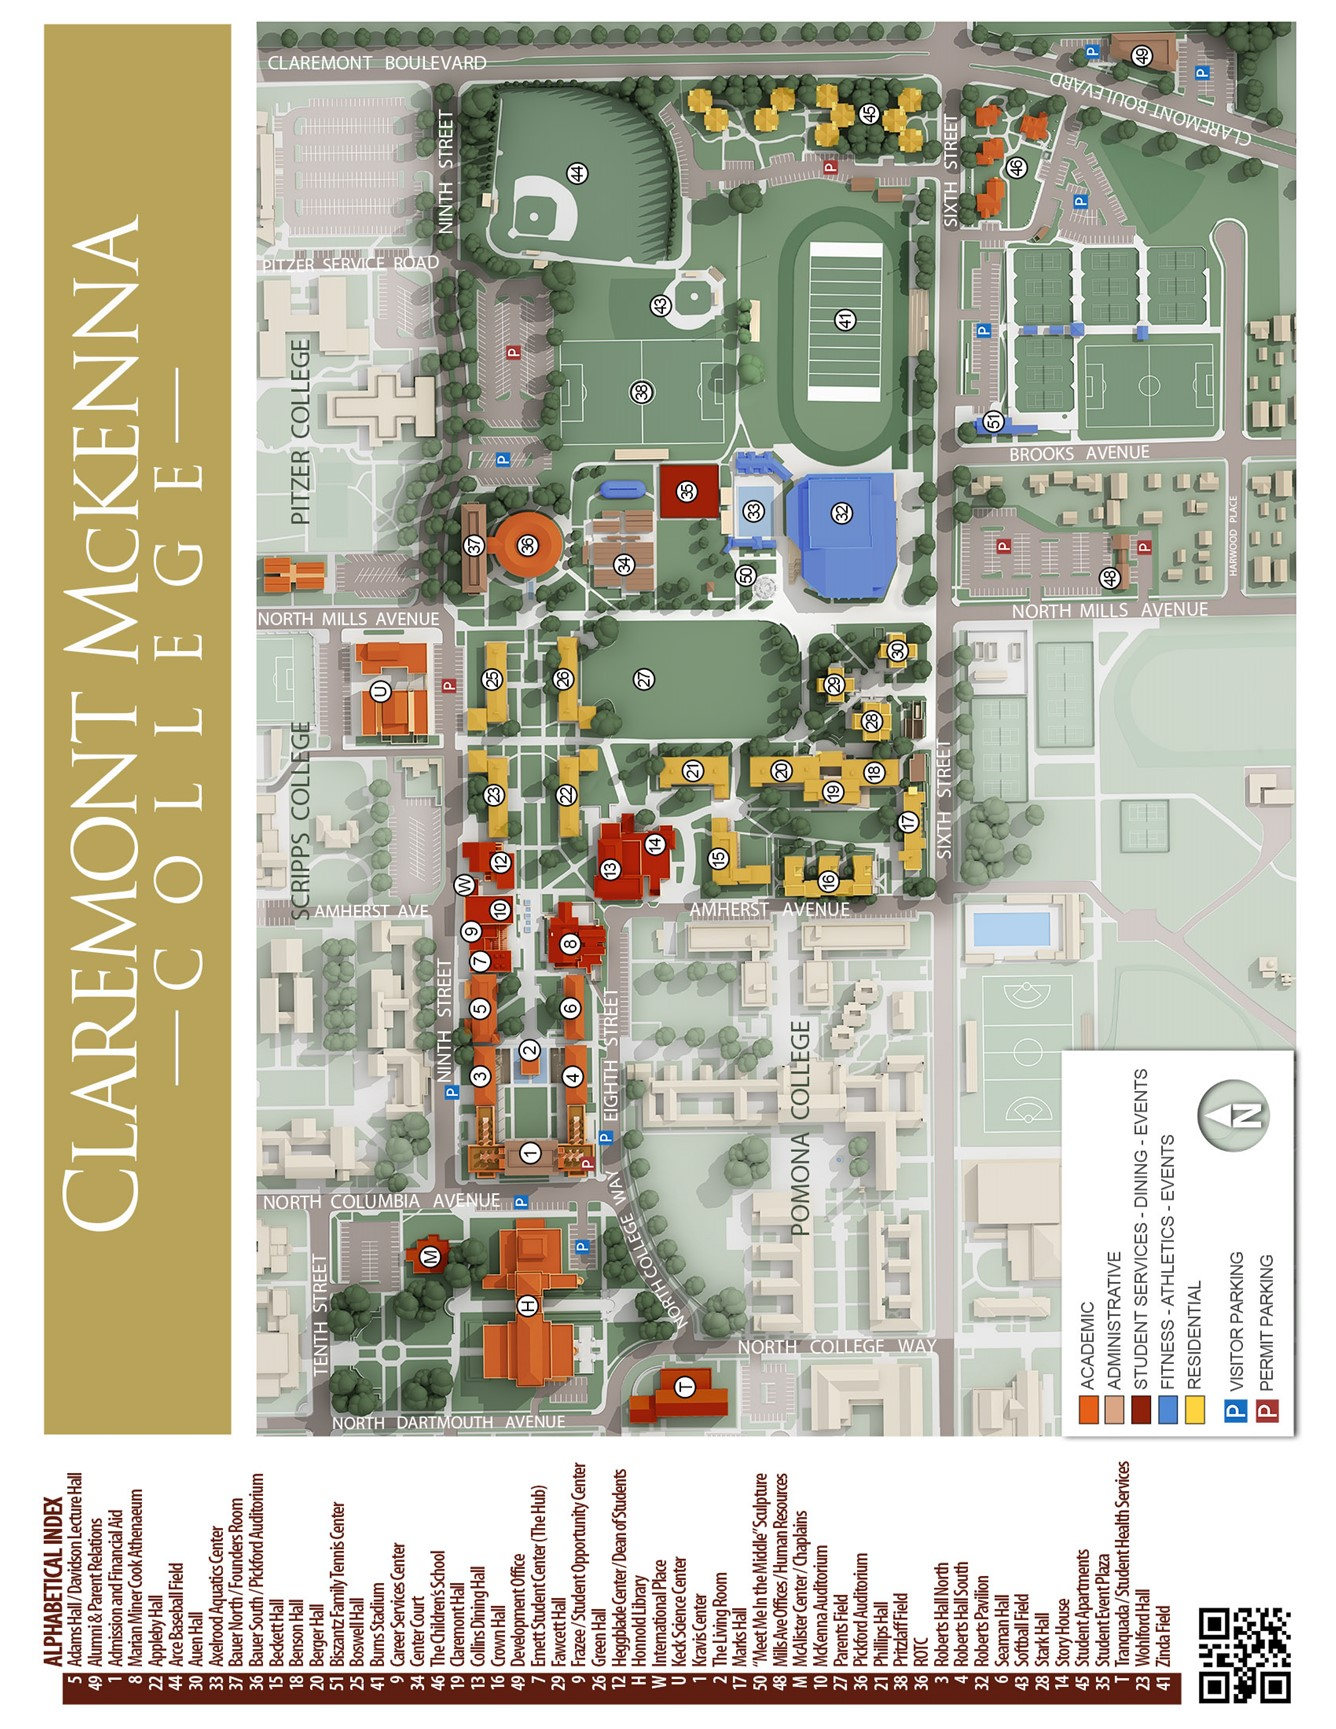
\includegraphics{https://raw.githubusercontent.com/CMC-QCL/fellow-handbook/main/Images/Claremont_Map.jpg?token=GHSAT0AAAAAABSRTQJAEGK5UEDKUP2OUEZCYR2QPIQ}
\caption{Claremont Campus Map}
\end{figure}

\hypertarget{employee-materials}{%
\chapter{Employee Materials}\label{employee-materials}}

\begin{itemize}
\tightlist
\item[$\square$]
  Employee ID

  \begin{itemize}
  \tightlist
  \item[$\square$]
    Go to Connects in The Claremont Colleges Library Honnold Mudd (H on map, page 4)

    \begin{itemize}
    \tightlist
    \item[$\square$]
      Take picture
    \item[$\square$]
      Receive ID
    \end{itemize}
  \item[$\square$]
    Go to Story House (14 on map, page 4)

    \begin{itemize}
    \tightlist
    \item[$\square$]
      Get access to infrastructure (doors)
    \item[$\square$]
      Also need a KEY for office room
    \end{itemize}
  \end{itemize}
\item[$\square$]
  Email and Username

  \begin{itemize}
  \tightlist
  \item[$\square$]
    Setup appointment for IT (Jeff)

    \begin{itemize}
    \tightlist
    \item[$\square$]
      \href{mailto:Jeffrey.Ng@claremontmckenna.edu}{\nolinkurl{Jeffrey.Ng@claremontmckenna.edu}} (\href{mailto:jng@cmc.edu}{\nolinkurl{jng@cmc.edu}}) or \href{mailto:help@cmc.edu}{\nolinkurl{help@cmc.edu}}
    \end{itemize}
  \item[$\square$]
    Obtain computer access
  \item[$\square$]
    Get put into system
  \end{itemize}
\item[$\square$]
  Kronos

  \begin{itemize}
  \tightlist
  \item[$\square$]
    Send email to Payroll

    \begin{itemize}
    \tightlist
    \item[$\square$]
      \href{mailto:payroll@cmc.edu}{\nolinkurl{payroll@cmc.edu}}
    \end{itemize}
  \item[$\square$]
    Find Kronos in Workday
  \item[$\square$]
    Log in hours

    \begin{itemize}
    \tightlist
    \item[$\square$]
      Talk to Janna
    \end{itemize}
  \end{itemize}
\item[$\square$]
  Health Documents

  \begin{itemize}
  \tightlist
  \item[$\square$]
    \url{https://www.cmc.edu/healthscreen}
  \end{itemize}
\item[$\square$]
  Training with EVERFI

  \begin{itemize}
  \tightlist
  \item[$\square$]
    Hazard Communication (CA)
  \item[$\square$]
    Protecting Youth
  \item[$\square$]
    Preventing Harassment and Discrimination: Non-Supervisors
  \item[$\square$]
    Injury \& Illness Prevention
  \item[$\square$]
    Data Security and Privacy
  \end{itemize}
\end{itemize}

\hypertarget{accounts-and-software}{%
\chapter{Accounts and Software}\label{accounts-and-software}}

\begin{itemize}
\tightlist
\item
  CMC Self-Service Account Management

  \begin{itemize}
  \tightlist
  \item
    \url{https://mypassword.claremontmckenna.edu/showLogin.cc}\strut \\
  \end{itemize}
\item
  CMC Email

  \begin{itemize}
  \tightlist
  \item
    \url{https://cmc.edu/mail/office365}

    \begin{itemize}
    \tightlist
    \item
      CMC e-mail address: \href{mailto:firstname.lastname@claremontmckenna.edu}{\nolinkurl{firstname.lastname@claremontmckenna.edu}}\\
    \item
      Short-hand: \href{mailto:firstthreelettersofyourfirstnameandwholelastname@cmc.edu}{\nolinkurl{firstthreelettersofyourfirstnameandwholelastname@cmc.edu}}\\
    \end{itemize}
  \end{itemize}
\item
  Dashboards Events

  \begin{itemize}
  \tightlist
  \item
    \url{https://events.cmc.edu/newemployeeusername/home}\strut \\
  \end{itemize}
\item
  GitHub

  \begin{itemize}
  \tightlist
  \item
    \url{https://github.com/CMC-QCL}\strut \\
  \end{itemize}
\item
  Workday

  \begin{itemize}
  \tightlist
  \item
    \url{https://www.myworkday.com/theclaremontcolleges/d/home.htmld} (refer to page 3)\\
  \item
    Kronos (in here)\\
  \end{itemize}
\item
  QCL Home page

  \begin{itemize}
  \tightlist
  \item
    cmc.edu/login\\
  \item
    \url{https://www.cmc.edu/qcl}\strut \\
  \end{itemize}
\item
  Box

  \begin{itemize}
  \tightlist
  \item
    \url{https://claremontmckenna.account.box.com/login?redirect_url=\%2Ffolder\%2F0}\strut \\
  \end{itemize}
\item
  Bit.ly

  \begin{itemize}
  \tightlist
  \item
    No account (you will use it a lot)\\
  \item
    \url{https://bitly.com/}\strut \\
  \end{itemize}
\item
  Qualtrics

  \begin{itemize}
  \tightlist
  \item
    \url{https://qfreeaccountssjc1.az1.qualtrics.com/login?path=\%2FQ\%2FMyProjectsSection\&product=project-store-proxy}\strut \\
  \end{itemize}
\item
  Localist

  \begin{itemize}
  \tightlist
  \item
    \url{https://events.cmc.edu/admin}\strut \\
  \end{itemize}
\item
  Zoom

  \begin{itemize}
  \tightlist
  \item
    \url{https://cmc-its.zoom.us}\strut \\
  \end{itemize}
\item
  Teams

  \begin{itemize}
  \tightlist
  \item
    Make sure to download desktop version and mobile as well\\
  \item
    \url{https://teams.microsoft.com}\strut \\
  \end{itemize}
\item
  Instagram

  \begin{itemize}
  \tightlist
  \item
    \url{https://www.instagram.com/cmc.qcl/}
  \end{itemize}
\end{itemize}

\emph{Issues: contact another Graduate Fellow or IT (\href{mailto:help@cmc.edu}{\nolinkurl{help@cmc.edu}})}

\hypertarget{logins-and-passwords}{%
\chapter{Logins and Passwords}\label{logins-and-passwords}}

\begin{longtable}[]{@{}lcr@{}}
\toprule
Accounts & Username & Password \\
\midrule
\endhead
CMC Self-Service Account Management & & \\
CMC Email & & \\
Dashboards Events & & \\
GitHub & & \\
Workday & & \\
QCL Home page & & \\
Box & & \\
Bit.ly & & \\
Qualtrics & & \\
Localist & & \\
Zoom & & \\
Teams & & \\
Instagram & & \\
\bottomrule
\end{longtable}

\emph{Firefox: bookmark websites}

\hypertarget{schedule}{%
\chapter{Schedule}\label{schedule}}

\textbf{Important Dates}

\begin{itemize}
\tightlist
\item
  Team meetings

  \begin{itemize}
  \tightlist
  \item
    Biweekly: Wednesdays 10am -11am\\
  \end{itemize}
\item
  Graduate Fellow meetings

  \begin{itemize}
  \tightlist
  \item
    Talk to Dr.~Park to set up best time\\
  \item
    Current Fellow meeting: 9:30am-10am\\
  \item
    New Time: \_\_\_\_\_\_\_\_\_\_\_\_\_\_\_\_\_\_\_\_\_\_\_\\
  \end{itemize}
\item
  Workshops

  \begin{itemize}
  \tightlist
  \item
    Wednesdays 3pm-5pm or 4pm-6pm\\
  \item
    Fridays 9am-11am or 10am-12pm\\
  \end{itemize}
\item
  Staff days

  \begin{itemize}
  \tightlist
  \item
    Janna will send out email\\
  \end{itemize}
\item
  Employees Schedule (20 hours a week)

  \begin{itemize}
  \tightlist
  \item
    Talk to Dr.~Park
  \end{itemize}
\end{itemize}

\begin{longtable}[]{@{}
  >{\raggedright\arraybackslash}p{(\columnwidth - 8\tabcolsep) * \real{0.1667}}
  >{\centering\arraybackslash}p{(\columnwidth - 8\tabcolsep) * \real{0.2143}}
  >{\centering\arraybackslash}p{(\columnwidth - 8\tabcolsep) * \real{0.2381}}
  >{\centering\arraybackslash}p{(\columnwidth - 8\tabcolsep) * \real{0.2143}}
  >{\raggedleft\arraybackslash}p{(\columnwidth - 8\tabcolsep) * \real{0.1667}}@{}}
\toprule
\begin{minipage}[b]{\linewidth}\raggedright
Monday
\end{minipage} & \begin{minipage}[b]{\linewidth}\centering
Tuesday
\end{minipage} & \begin{minipage}[b]{\linewidth}\centering
Wednesday
\end{minipage} & \begin{minipage}[b]{\linewidth}\centering
Thursday
\end{minipage} & \begin{minipage}[b]{\linewidth}\raggedleft
Friday
\end{minipage} \\
\midrule
\endhead
Workshop: 5pm -- 7pm & Current Fellow meeting: 9:30am-10am & Biweekly Team meeting: 10am -11am & & Workshop: 10am-12pm \\
\bottomrule
\end{longtable}

\emph{Days off: Holidays and Academic break}

\hypertarget{graduate-fellows-meeting}{%
\chapter{Graduate Fellows Meeting}\label{graduate-fellows-meeting}}

\begin{itemize}
\tightlist
\item
  BOX

  \begin{itemize}
  \tightlist
  \item
    Titled: QCL Fellows Meeting Agenda\\
  \item
    \url{https://claremontmckenna.app.box.com/folder/0}
  \end{itemize}
\end{itemize}

\begin{figure}
\centering
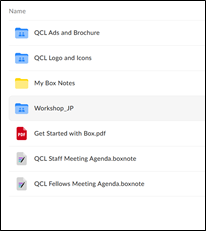
\includegraphics{https://raw.githubusercontent.com/CMC-QCL/fellow-handbook/main/Images/Picture2.png?token=GHSAT0AAAAAABQHYZSEQDK54EPONUMMGKSUYR2TXCQ}
\caption{QCL Fellows Meeting Agenda}
\end{figure}

\begin{itemize}
\tightlist
\item
  Agenda

  \begin{itemize}
  \tightlist
  \item
    Write meeting notes

    \begin{itemize}
    \tightlist
    \item
      Before meeting

      \begin{itemize}
      \tightlist
      \item
        Let Dr.~Park write minutes unless he asks you\\
      \end{itemize}
    \end{itemize}
  \item
    Follow along in the meeting\\
  \item
    TO DOs

    \begin{itemize}
    \tightlist
    \item
      Your assignments for the week
    \end{itemize}
  \end{itemize}
\end{itemize}

\begin{figure}
\centering
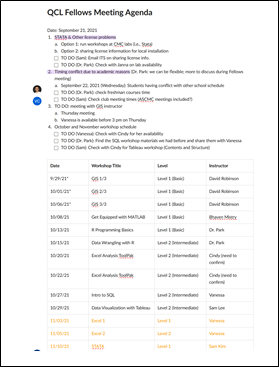
\includegraphics{https://raw.githubusercontent.com/CMC-QCL/fellow-handbook/main/Images/Picture3.png?token=GHSAT0AAAAAABQHYZSEVEDCJCUX63ECFNBCYR2TYKQ}
\caption{Your assignments for the week}
\end{figure}

\hypertarget{editing-the-qcl-cmc-website}{%
\chapter{Editing the QCL-CMC Website}\label{editing-the-qcl-cmc-website}}

Every week, we update cmc.edu/qcl/qcl-workshop page, whenever we open or close registration + update our schedule

In terms of website access:

\begin{enumerate}
\def\labelenumi{\arabic{enumi}.}
\tightlist
\item
  Log in at cmc.edu/login
\item
  Go to cmc.edu/qcl
\item
  See ``View,'' ``Edit,'' and ``Revisions'' tabs right above body
\end{enumerate}

\begin{figure}
\centering

\includegraphics{https://raw.githubusercontent.com/CMC-QCL/fellow-handbook/main/Images/Picture4.png?token=GHSAT0AAAAAABQHYZSF4AJT2DLWNTMO2VOKYR2TZUQ}
\caption{website access}
\end{figure}

\hypertarget{workshops}{%
\chapter{Workshops}\label{workshops}}

\hypertarget{a.-start-of-semester}{%
\subsubsection{\texorpdfstring{a. Start of Semester }{a. Start of Semester }}\label{a.-start-of-semester}}

\begin{itemize}
\tightlist
\item
  Topics

  \begin{itemize}
  \tightlist
  \item
    Pick
  \item
    Dr.~Park in Fellows meeting
  \end{itemize}
\item
  Dates

  \begin{itemize}
  \tightlist
  \item
    Assign
  \item
    Dr.~Park in Fellows meeting
  \end{itemize}
\item
  Instructors

  \begin{itemize}
  \tightlist
  \item
    Assign
  \item
    Dr.~Park in Fellows meeting
  \end{itemize}
\end{itemize}

\hypertarget{b.-possible-workshops}{%
\subsubsection{\texorpdfstring{b. Possible Workshops }{b. Possible Workshops }}\label{b.-possible-workshops}}

\begin{itemize}
\tightlist
\item
  Dr.~Park

  \begin{itemize}
  \tightlist
  \item
    R Programming Basics (level 1)\\
  \item
    Data Wrangling with R (level 2)
  \item
    Tableau (level 1)\\
  \end{itemize}
\item
  Bhaven

  \begin{itemize}
  \tightlist
  \item
    Get Equipped with LaTeX (level 1)\\
  \item
    Get Equipped with MATLAB (level 1)\\
  \end{itemize}
\item
  Vanessa

  \begin{itemize}
  \tightlist
  \item
    Excel (level 1)\\
  \item
    SQL (level 1) (Find cloud based complier that imports files like csv and sql)
  \item
    GIS (level 1) (ArcGIS Online for Mac and Windows)
  \end{itemize}
\item
  Sam Kim

  \begin{itemize}
  \tightlist
  \item
    STATA (level 1)
  \item
    STATA (level 2) -- develop with Sam Lee
  \end{itemize}
\item
  Others (need instructors)

  \begin{itemize}
  \tightlist
  \item
    Julia = Alfonso Landeros \href{mailto:alanderos@ucla.edu}{\nolinkurl{alanderos@ucla.edu}}
  \item
    XSEDE
  \item
    Bash = Brad McCauley \href{mailto:bmccauley@hmc.edu}{\nolinkurl{bmccauley@hmc.edu}}
  \item
    Unix Shell and Git = Jeanine Finn \href{mailto:jeanine.finn@claremont.edu}{\nolinkurl{jeanine.finn@claremont.edu}}
  \item
    MS Power Automate as Pre to Power BI = Cindy Cheng \href{mailto:cindy.cheng@cgu.edu}{\nolinkurl{cindy.cheng@cgu.edu}}
  \item
    MS Power Query as Pre to Power BI = Cindy Cheng \href{mailto:cindy.cheng@cgu.edu}{\nolinkurl{cindy.cheng@cgu.edu}}
  \item
    Alteryx = Brandon Bak \href{mailto:brandonbak@gmail.com}{\nolinkurl{brandonbak@gmail.com}}
  \item
    Machine Learning = Aashita Kesarwani \href{mailto:akesarwani@hmc.edu}{\nolinkurl{akesarwani@hmc.edu}}
  \item
    Python
  \item
    Power BI = Jillian Seymour
  \end{itemize}
\end{itemize}

\hypertarget{c.-confirming-dates-with-instructors}{%
\subsubsection{\texorpdfstring{c.~Confirming Dates with Instructors }{c.~Confirming Dates with Instructors }}\label{c.-confirming-dates-with-instructors}}

Subject: QCL Workshops - confirming dates

Good afternoon Bhaven,

Happy Tuesday! I hope you are doing well! As the new semester approaches, I wanted to confirm if these dates work for you to instruct:

Monday, January 24, 2022, at 5pm - 7pm for Get Equipped with LaTeX as an online workshop

Monday, February 21, 2022, at 5pm - 7pm for Get Equipped with MATLAB (TBA as a hybrid, in-person, or online workshop due to the Covid policies)

We have only scheduled up to Spring Break, I will have to follow up in the future for the rest of the semester's dates. Do these dates and time work for you to instruct the workshops?

Thank you,\\
Vanessa Arias Casillas\\
Graduate Fellow - Murty Sunak Quantitative and Computing Lab (QCL)\\
Claremont Mckenna College\\
\href{mailto:vanessa.casillas@claremontmckenna.edu}{\nolinkurl{vanessa.casillas@claremontmckenna.edu}}

\begin{center}\rule{0.5\linewidth}{0.5pt}\end{center}

\hypertarget{d.-worksflow}{%
\subsubsection{\texorpdfstring{d.~Worksflow }{d.~Worksflow }}\label{d.-worksflow}}

\hypertarget{two-weeks-before-day-of-workshop}{%
\subsubsection{\texorpdfstring{Two weeks before day of workshop }{Two weeks before day of workshop }}\label{two-weeks-before-day-of-workshop}}

\begin{itemize}
\tightlist
\item
  Contact Instructor\\
\item
  Setup meeting

  \begin{itemize}
  \tightlist
  \item
    Agenda of meeting
  \item
    Summary of localist
  \item
    Software
  \item
    Websites
  \item
    Licenses
  \end{itemize}
\end{itemize}

\textbf{\emph{Instructors Notes turned into Summaries}}

Good afternoon {[}instructor's name{]},

Happy Tuesday! I am looking forward to your dryrun of {[}workshop{]}! I am starting to create the registration page for the workshop and would like to get a bit of information from you about the workshop.

First, do you have a summary page for your workshop? I have an example of Sam Lee's below:

\begin{figure}
\centering
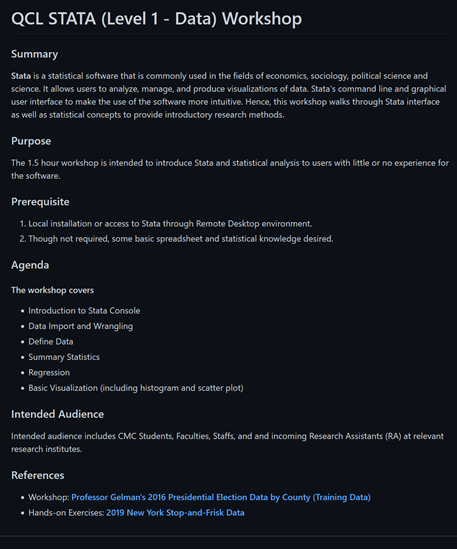
\includegraphics{https://raw.githubusercontent.com/CMC-QCL/fellow-handbook/main/Images/Picture5.png?token=GHSAT0AAAAAABQHYZSEHQGEXMFLADQ7N6KUYR2T32A}
\caption{example of Sam Lee's}
\end{figure}

Second, do you have any pre-workshop requirements that the attendees need to do before the workshop? Like download programs or sign up for a license.\\
Third, what time did you want to do your workshop at 3pm-5pm or 4pm-6pm?\\
Fourth, would you like this workshop to be a hybrid, online only or in-person only?\\
Lastly, is there any information you would like me to let the attendees know about before walking into the workshop? like website where to download files or a note about the data.\\
Thank you for this information, it will help me in getting the workshop's registration ready.

Thank you,\\
Graduate Fellow - Murty Sunak Quantitative and Computing Lab (QCL)

\textbf{\emph{{[}QCL Workshop{]} Title}}

About this Event\\
Title\\
Summary\\
Agenda:\\
Learning Objectives: (You will learn how to)\\
Prerequisite:\\
Location:\\
Participants:

\textbf{\emph{Example Instructors Notes turned into Summaries}}

\emph{{[}QCL Workshop{]} R Programming Basics (Level 1 -- Coding)}

About this Event

R Programming Basics (Level 1 - Coding)

Summary:\\
R is an open-source statistical programming language. R is widely used in industry as well as in academia for statistical analysis and data visualization. In this workshop, we introduce the basics of the R language and its programming environment through simple hands-on examples.
This workshop is designed for beginners in R programming, so no prior knowledge of R programming is needed. However, general programming knowledge in any programming language will be help understand the programming concepts.
We will be using RStudio Cloud for hands-on. Please create a free account at \url{https://rstudio.cloud} before join the workshop.

Agenda:\\
• Basics of R and RStudio
• R Programming Environment: Workspace, Working Directory, Package
• R objects (data structure and function)
• R packages for data import and export
• R graphics for simple plotting methods
• Basic statistical analysis using R

Location:\\
Hybrid (In-person: QCL Classroom, Online: Zoom information will be provided to the attendees after registration)
Click here to find your way to the QCL.

Participants:\\
CMC Students, Faculty, and Staff\\
\_\_\_

\emph{Data Wrangling with R (Level 2 - Data)}

Summary:\\
Data wrangling is the process of obtaining, cleaning, reshaping, and transforming raw (and messy) data into a useable form of processed (and tidy) data. It is known that a majority of data analysts and data scientists spend as much as 80\% of their time on data wrangling. So it's essential to get familiar with good data wrangling tools that help you save time and avoid errors. In this hands-on workshop, you will learn basic skills to import, export, clean, reshape, transform, and visualize data using well-known data science package called tidyverse.

Learning Objectives: (You will learn how to)\\
Import and export data
Clean, reshape and transform data
Make messy data into tidy data
Visualize tidy data using ggplot2 (if time permits)

Prerequisites:\\
Basic knowledge of R and RStudio (e.g., R Programming for Beginners - Level 1)
RStudio Cloud account; if you don't have one yet, please create a new account from \url{https://rstudio.cloud} site.
Tidyverse package; please make sure that you have installed the tidyverse package in your R environment. See \url{https://www.tidyverse.org} for more information.

Location:\\
Hybrid (In-person: QCL Classroom, Online: Zoom information will be provided to the attendees after registration)
Click here to find your way to the QCL.

Participants:\\
CMC Students, Faculty, and Staff\\
\_\_\_

\emph{GIS - Part 2 (Level 1 - Data) Workshop}

About this Event

Summary:\\
This workshop will introduce you to the ever-expanding and fascinating world of geographic information systems (GIS). In three 2-hour sessions you will learn about what GIS is, how it is used in a multitude of industries and fields, and how to get started using GIS software. We will examine GIS concepts and software tools used to visualize real-world features, discover patterns, and communicate information. Primarily using ArcGIS Online (if you can hyperlink: \url{https://doc.arcgis.com/en/arcgis-online/get-started/what-is-agol.htm}) you will work with GIS maps, explore data, and analyze maps and data as you learn fundamental concepts that underlie GIS technology.
Through a series of presentations, in-class tutorials, and homework assignments this workshop will give you a strong beginning foundation on how to make maps and explore spatial data to identify patterns and insights in your data you never knew possible. You will come away from this workshop with the understanding you need to start working with GIS and utilize it in your own work and explorations. You do not need any previous experience -- just your own curiosity!
Students in this workshop (in fact, all Claremont Colleges students) have free access to a wide variety Esri GIS products. For more information, check out the Claremont Colleges Library Geographic Information System (GIS) Services home page, \url{https://library.claremont.edu/gis/}

Learning Objectives: (You will learn how to)\\
Topics will include:
• Introduction to the GIS Platform
• Theoretical basis of GIS and the Geographic Approach
• What can you do with GIS?
• Understanding GIS data
• An introduction to Coordinate systems and Projections
• Acquiring and selecting GIS Data
• Utilizing and preparing your own data for GIS
• Creating maps -- basic cartography, symbology
• The US Census and GIS
• Introductory Spatial Analysis
• Sharing results -- physical maps and the world online maps

Location:\\
The following event will be conducted in a hybrid format:
• Virtual: Zoom
• In-Person: QCL Classroom

Participants:\\
7C Students, Faculty and Staff\\
\_\_\_

\hypertarget{one-week-before-day-of-workshop}{%
\subsubsection{\texorpdfstring{One week before day of workshop }{One week before day of workshop }}\label{one-week-before-day-of-workshop}}

\textbf{Moderator}

\begin{itemize}
\tightlist
\item
  If you are instructing

  \begin{itemize}
  \tightlist
  \item
    Ask for whoever moderator a week before or instruct and moderate yourself.
  \end{itemize}
\end{itemize}

\textbf{Zoom}

Step 1:

\begin{itemize}
\tightlist
\item
  Go to meetings\\
  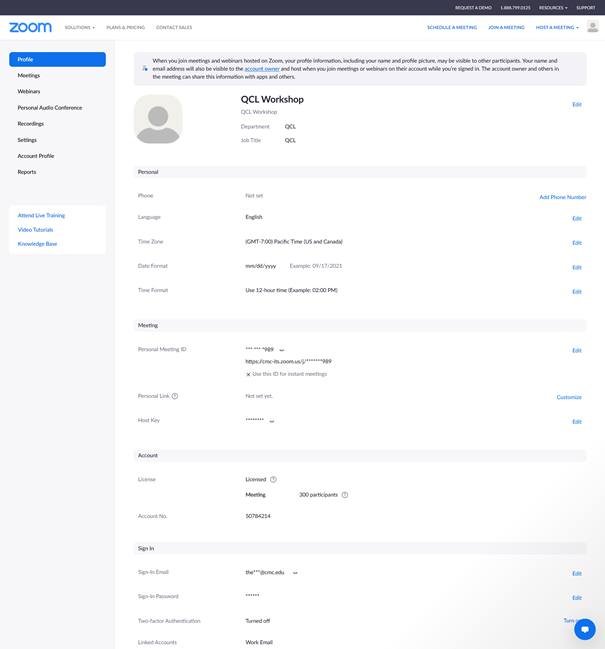
\includegraphics{https://raw.githubusercontent.com/CMC-QCL/fellow-handbook/main/Images/Picture6.png?token=GHSAT0AAAAAABQHYZSE6MSJ2F3BFWBHTLK6YR2U27Q}
\end{itemize}

Step 2:

\begin{itemize}
\tightlist
\item
  Click on Schedule\\
  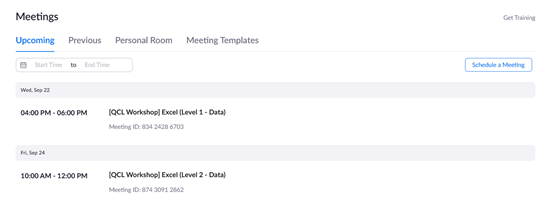
\includegraphics{https://raw.githubusercontent.com/CMC-QCL/fellow-handbook/main/Images/Picture7.png?token=GHSAT0AAAAAABQHYZSEXEJ7Y5WPF3OJWSSYYR2U6CQ}
\end{itemize}

Step 3:

\begin{itemize}
\tightlist
\item
  Go to QCL workshop\\
  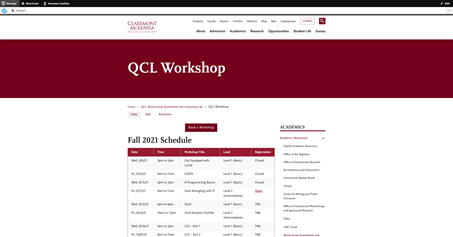
\includegraphics{https://raw.githubusercontent.com/CMC-QCL/fellow-handbook/main/Images/Picture8.png?token=GHSAT0AAAAAABQHYZSFXW3ZERAF3VRPK2TSYR2U6DQ}
\end{itemize}

Step 4:

\begin{itemize}
\tightlist
\item
  Look for workshop you are working\\
  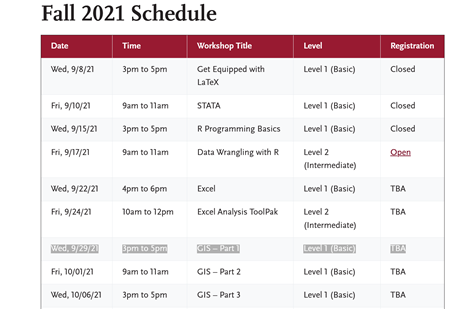
\includegraphics{https://raw.githubusercontent.com/CMC-QCL/fellow-handbook/main/Images/Picture9.png?token=GHSAT0AAAAAABQHYZSEUEWGYDWYUKRSQ42OYR2U6EA}
\end{itemize}

Step 5:

\begin{itemize}
\tightlist
\item
  Fill in meeting information on Zoom then click save,

  \begin{itemize}
  \tightlist
  \item
    Description (Optional) comes from Instructor's meeting\\
    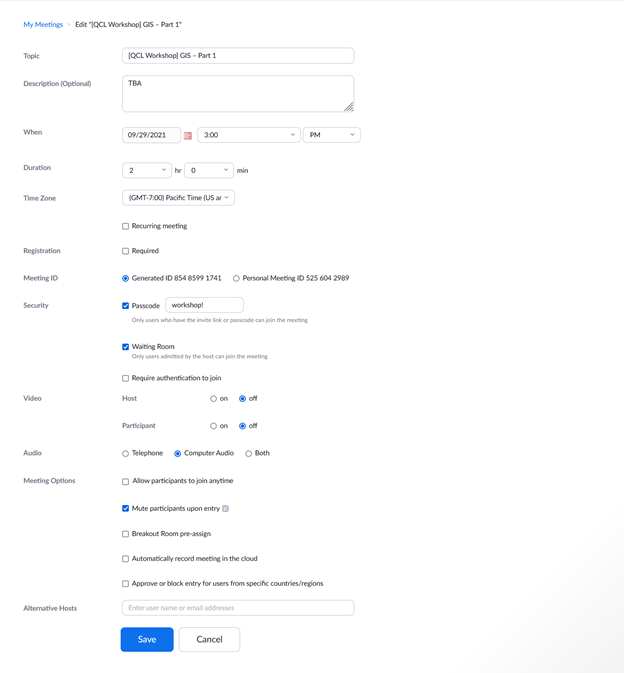
\includegraphics{https://raw.githubusercontent.com/CMC-QCL/fellow-handbook/main/Images/Picture10.png?token=GHSAT0AAAAAABQHYZSFVUDX4IYQ6FDYW256YR2U6FQ}
  \end{itemize}
\end{itemize}

Step 6:

\begin{itemize}
\tightlist
\item
  You will see this\\
  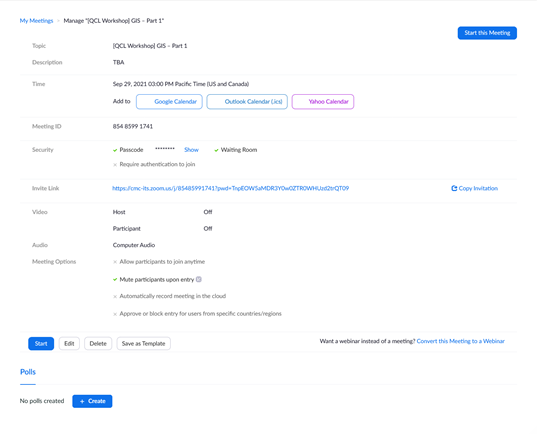
\includegraphics{https://raw.githubusercontent.com/CMC-QCL/fellow-handbook/main/Images/Picture11.png?token=GHSAT0AAAAAABQHYZSFAEJN323XN3CR6QHYYR2U6GA}
\end{itemize}

Step 7:

\begin{itemize}
\tightlist
\item
  On meeting tab, it should there\\
  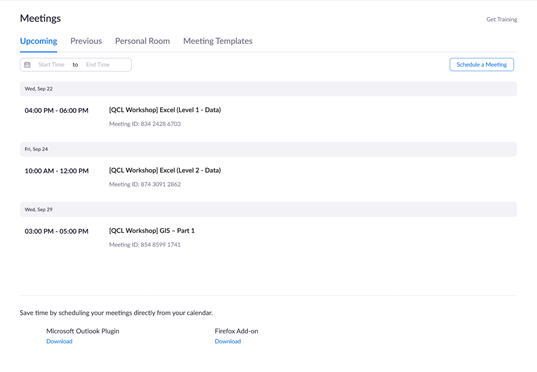
\includegraphics{https://raw.githubusercontent.com/CMC-QCL/fellow-handbook/main/Images/Picture12.png?token=GHSAT0AAAAAABQHYZSEFGAFFKTHWSTTNBROYR2U6GQ}
\end{itemize}

\textbf{Localist}

Step 1:

\begin{itemize}
\tightlist
\item
  Start by copying an old event

  \begin{itemize}
  \tightlist
  \item
    Make sure you are working on copy\\
  \end{itemize}
\item
  Fill in all information (Like below)

  \begin{itemize}
  \tightlist
  \item
    Click ``Include Above in Schedule''\\
  \item
    Delete the old Confirmed dates\\
  \item
    Description is made from Instructor's meeting\\
    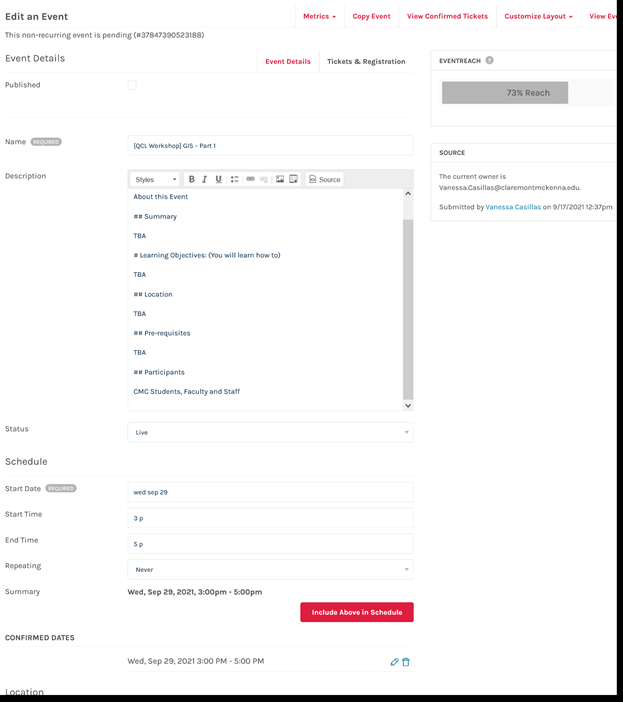
\includegraphics{https://raw.githubusercontent.com/CMC-QCL/fellow-handbook/main/Images/Localist1.png?token=GHSAT0AAAAAABQHYZSEYOLQEPQKD6PN5JPUYR2WIPA}
  \end{itemize}
\end{itemize}

Step 2:

\begin{itemize}
\tightlist
\item
  Fill out Location (Like below)

  \begin{itemize}
  \tightlist
  \item
    Check if event is only in-person, only virtual or hybrid\\
    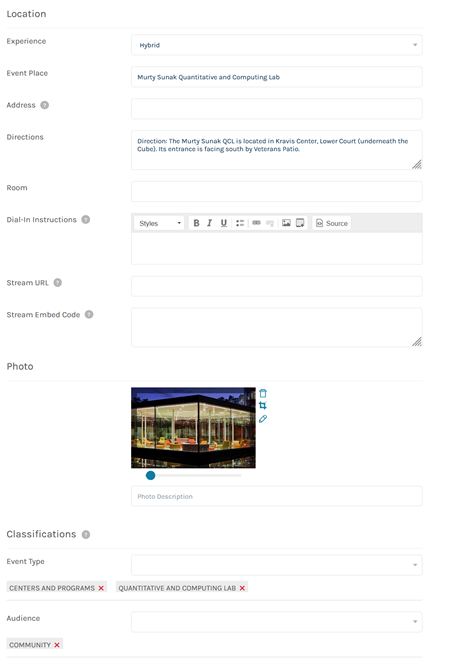
\includegraphics{https://raw.githubusercontent.com/CMC-QCL/fellow-handbook/main/Images/Localist2.png?token=GHSAT0AAAAAABQHYZSFXDDAUR7NYQXKVMJYYR2WIPQ}
  \end{itemize}
\end{itemize}

Step 3:

\begin{itemize}
\tightlist
\item
  Change the Owner to yourself

  \begin{itemize}
  \tightlist
  \item
    Check Vanity URL (qcl\_workshop\_stata\_fa21\_1117)\\
    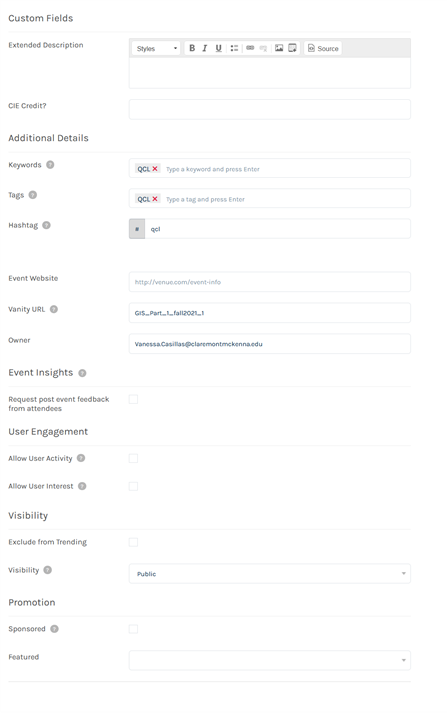
\includegraphics{https://raw.githubusercontent.com/CMC-QCL/fellow-handbook/main/Images/Localist3.png?token=GHSAT0AAAAAABQHYZSFDUBBM4CG6GSGGT2IYR2WIQA}
  \end{itemize}
\end{itemize}

Step 4:

\begin{itemize}
\tightlist
\item
  Add a Ticket Types

  \begin{itemize}
  \tightlist
  \item
    Virtual or In-Person (or both)\\
  \item
    Make sure Virtual is always on Top\\
    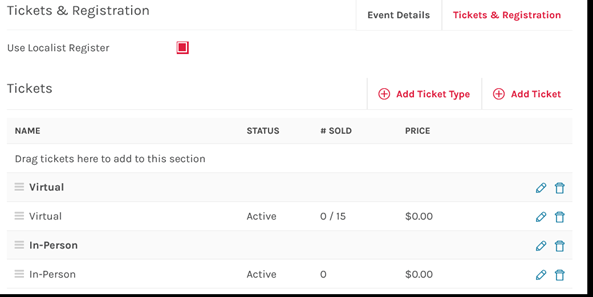
\includegraphics{https://raw.githubusercontent.com/CMC-QCL/fellow-handbook/main/Images/Localist4.png?token=GHSAT0AAAAAABQHYZSF7V6AEFIP5R4PXNAIYR2WIQQ}
  \end{itemize}
\end{itemize}

Step 5:

\begin{itemize}
\tightlist
\item
  Add a Virtual ticket name is ZOOM and drag to the right ticket type (pic wrong)

  \begin{itemize}
  \tightlist
  \item
    Then go into additional ticket options\\
    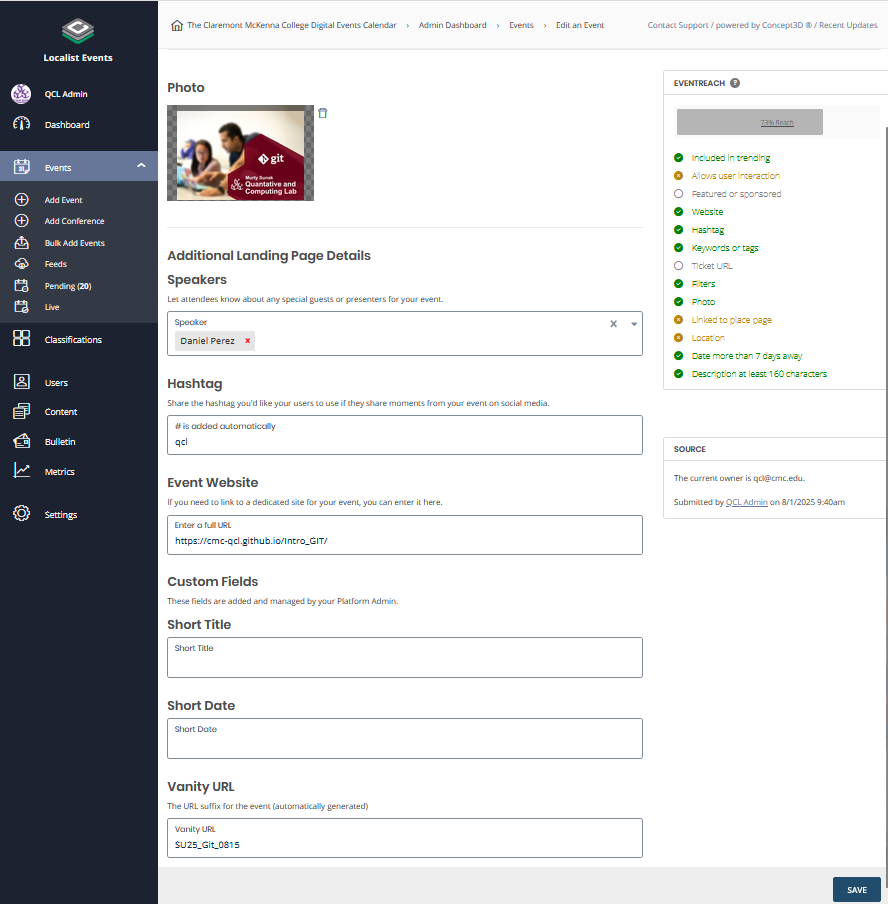
\includegraphics{https://raw.githubusercontent.com/CMC-QCL/fellow-handbook/main/Images/Localist5.png?token=GHSAT0AAAAAABQHYZSFVFO6FQGSCETFUZFEYR2WIRA}
  \end{itemize}
\end{itemize}

Step 6:

\begin{itemize}
\tightlist
\item
  Check to make sure settings are correct

  \begin{itemize}
  \tightlist
  \item
    Make sure Ticket availability dates correctly dated or left blank if you will manual turn off\\
    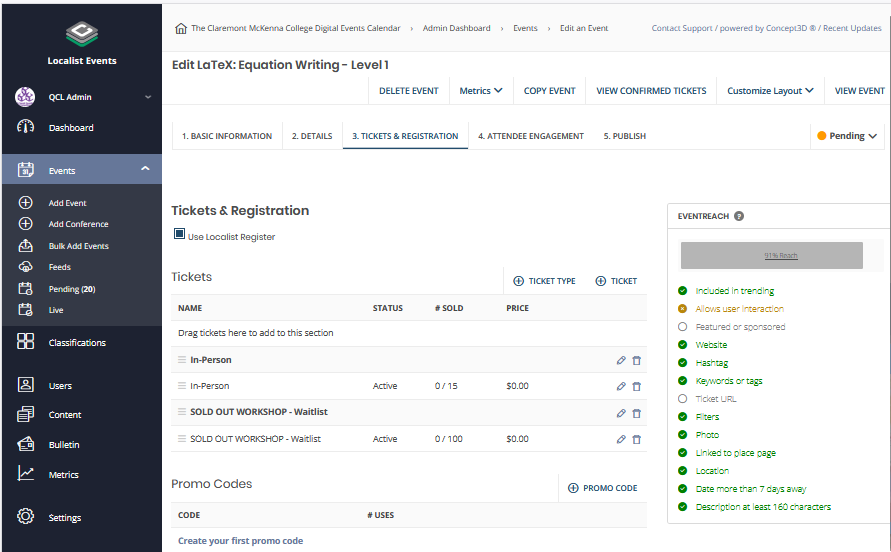
\includegraphics{https://raw.githubusercontent.com/CMC-QCL/fellow-handbook/main/Images/Localist6.png?token=GHSAT0AAAAAABQHYZSFOXZ54CXQFIHXBAZWYR2WIRQ}
  \end{itemize}
\end{itemize}

Step 7:

\begin{itemize}
\tightlist
\item
  Add in-person ticket named QCL CLASSROOM and drag to the right ticket type (pic wrong)

  \begin{itemize}
  \tightlist
  \item
    Then go into additional ticket options\\
    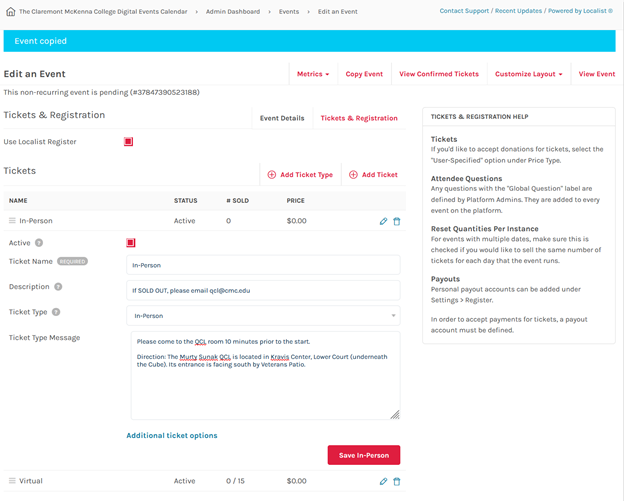
\includegraphics{https://raw.githubusercontent.com/CMC-QCL/fellow-handbook/main/Images/Localist7.png?token=GHSAT0AAAAAABQHYZSFLKHYDSMSDNSMEUWSYR2WISA}
  \end{itemize}
\end{itemize}

Step 8:

\begin{itemize}
\tightlist
\item
  Check to make sure setting are correct\\
  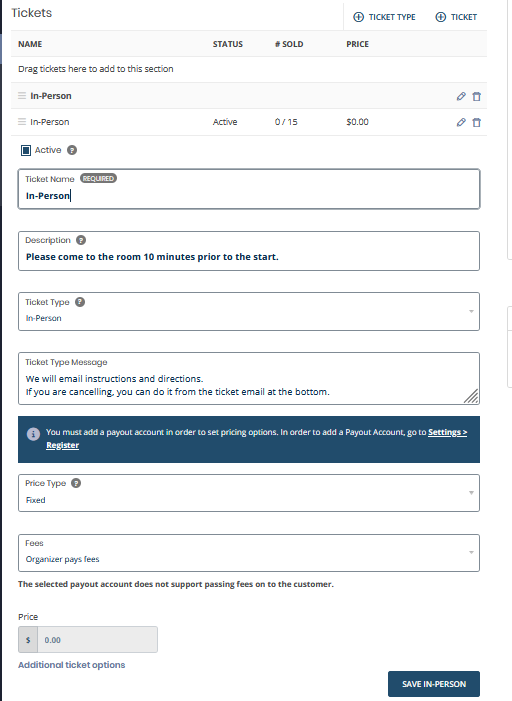
\includegraphics{https://raw.githubusercontent.com/CMC-QCL/fellow-handbook/main/Images/Localist8.png?token=GHSAT0AAAAAABQHYZSFRUQ6K25NP6NWHAISYR2WISQ}
\end{itemize}

Step 9:

\begin{itemize}
\tightlist
\item
  Check to make sure that Attendees Questions are correct
\end{itemize}

\begin{enumerate}
\def\labelenumi{\arabic{enumi}.}
\tightlist
\item
  ``Please enter your student ID \# (Must be 8 characters). For all faculty/staff/non-Claremont Colleges person, please insert 00000000.'' (Required)\\
\item
  ``Please indicate gender (male or female)''\\
\item
  ``Which one of the Claremont Colleges are you from?'' (Required)\\
\item
  ``If not from the Claremont Colleges, where are you from?''\\
\item
  ``Are you a Freshman, Sophomore, Junior, Senior, Graduate Student, Faculty, Staff or Other?'' (Required)\\
\item
  ``If Other, please specify:''\\
  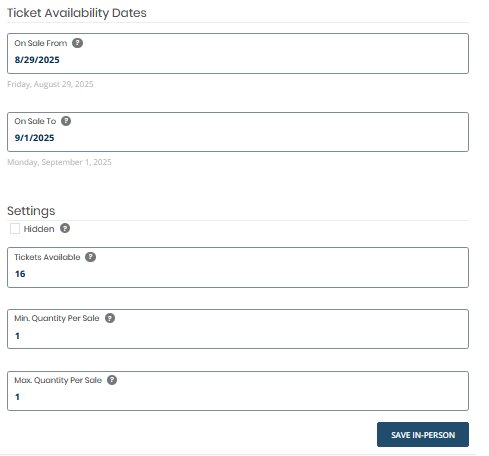
\includegraphics{https://raw.githubusercontent.com/CMC-QCL/fellow-handbook/main/Images/Localist9.png?token=GHSAT0AAAAAABQHYZSFAEB6X2GZ25OEQENGYR2WITA}
\end{enumerate}

Step 10:

\begin{itemize}
\tightlist
\item
  Check to make sure you have the correct Event Capacity\\
  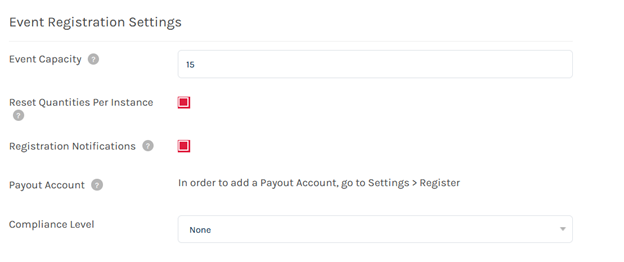
\includegraphics{https://raw.githubusercontent.com/CMC-QCL/fellow-handbook/main/Images/Lcoalist10.png?token=GHSAT0AAAAAABQHYZSFY5J3HMKLB776ILS2YR2WIVA}
\end{itemize}

Step 11:

\begin{itemize}
\tightlist
\item
  Publish or NOT

  \begin{itemize}
  \tightlist
  \item
    Make sure if you are publishing that the checkmark is checked\\
  \item
    But if you want another Fellow to review then make sure publish is not checked\\
  \item
    Then Click Save\\
  \end{itemize}
\item
  TEST! TEST! TEST!

  \begin{itemize}
  \tightlist
  \item
    when you set up the registration pages, please test them by registering for the workshops and see if everything works fine including the email confirmation, Zoom links, etc.\\
  \end{itemize}
\item
  Send Dr.~Park an email + post a message on Teams so that I can announce them.\\
  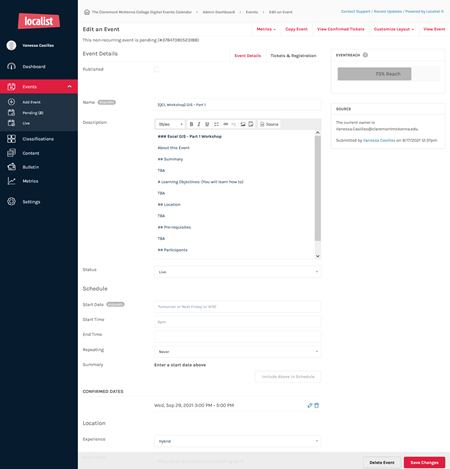
\includegraphics{https://raw.githubusercontent.com/CMC-QCL/fellow-handbook/main/Images/Localist11.png?token=GHSAT0AAAAAABQHYZSFOUTVRATRJCHFRTE6YR2WIWA}
\end{itemize}

\hypertarget{two-days-before-day-of-workshop}{%
\subsubsection{\texorpdfstring{Two days before day of workshop }{Two days before day of workshop }}\label{two-days-before-day-of-workshop}}

\emph{Close Registration for workshop}

Step 1:

\begin{itemize}
\tightlist
\item
  For those that do not require extensive prior prep, let's close them 5 pm a day before. And, 2 days prior for those that require requesting licenses

  \begin{itemize}
  \tightlist
  \item
    Go into event\\
  \item
    Go into tickets\\
  \item
    Click inactivate on any tickets that are active\\
    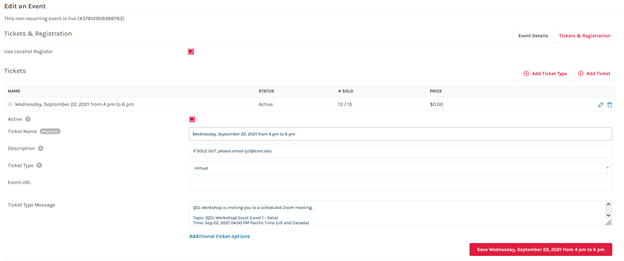
\includegraphics{https://raw.githubusercontent.com/CMC-QCL/fellow-handbook/main/Images/Twodays1.png?token=GHSAT0AAAAAABQHYZSEPWAA6NY4OZA7QJOEYR33BAQ}
  \end{itemize}
\end{itemize}

Step 2:

\begin{itemize}
\tightlist
\item
  You should see the ticket status as inactivate\\
  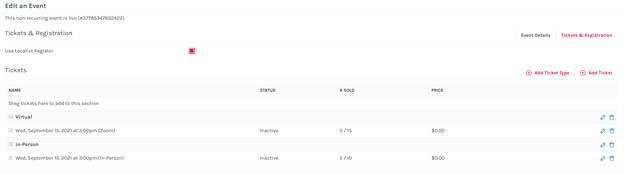
\includegraphics{https://raw.githubusercontent.com/CMC-QCL/fellow-handbook/main/Images/Twodays2.png?token=GHSAT0AAAAAABQHYZSEODR3PQ7UX5MCXLFGYR33BBQ}
\end{itemize}

\hypertarget{day-before-day-of-workshop}{%
\subsubsection{\texorpdfstring{Day before day of workshop }{Day before day of workshop }}\label{day-before-day-of-workshop}}

\textbf{Qualtrics}

Step 1:

\begin{itemize}
\tightlist
\item
  Make sure to make a Sign and Exit one

  \begin{itemize}
  \tightlist
  \item
    Make copy of old one\\
  \item
    Sign in for sign in (Fall\_2021\_Signin\_Survey\_SQL\_Lvl1\_Vanessa\_Casillas\_1119)\\
  \item
    Exit for Exit (Fall\_2021\_Exit\_Survey\_SQL\_Lvl1\_Vanessa\_Casillas\_1119)\\
    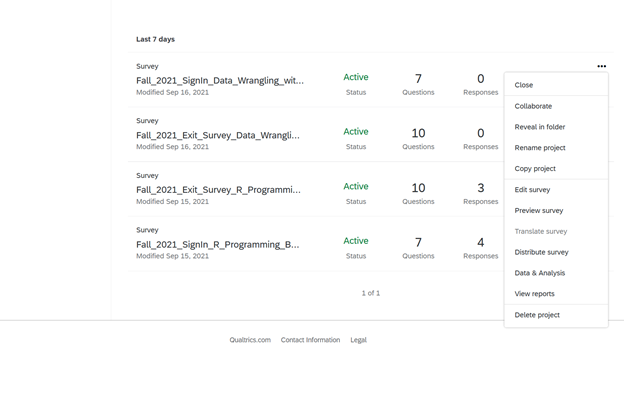
\includegraphics{https://raw.githubusercontent.com/CMC-QCL/fellow-handbook/main/Images/Qualtrics1.png?token=GHSAT0AAAAAABQHYZSELGZJGORAYQMXUJROYR33CZQ}
  \end{itemize}
\end{itemize}

Step 2:

\begin{itemize}
\tightlist
\item
  Change name to workshop name and instructor\\
  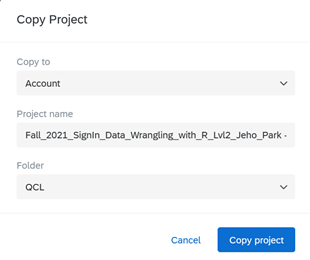
\includegraphics{https://raw.githubusercontent.com/CMC-QCL/fellow-handbook/main/Images/Qualtrics2.png?token=GHSAT0AAAAAABQHYZSFP26MDRYBTPC32QIAYR33C2A}
\end{itemize}

Step 3:

\begin{itemize}
\tightlist
\item
  Change workshop sign-in for and Date/Time

  \begin{itemize}
  \tightlist
  \item
    Sign-in\\
    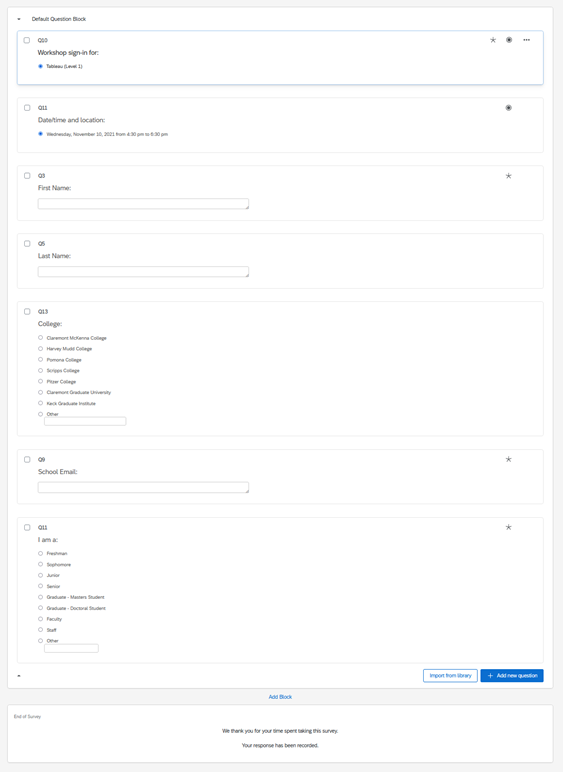
\includegraphics{https://raw.githubusercontent.com/CMC-QCL/fellow-handbook/main/Images/Qualtrics3.png?token=GHSAT0AAAAAABQHYZSEEVEODXVGSWBVS25EYR33C2Q}
  \end{itemize}
\end{itemize}

Step 4:

\begin{itemize}
\tightlist
\item
  Change workflow link

  \begin{itemize}
  \tightlist
  \item
    In email to the weird code\\
  \item
    Make sure Dr.~Park is getting an email sent to him\\
    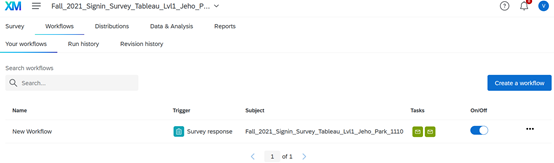
\includegraphics{https://raw.githubusercontent.com/CMC-QCL/fellow-handbook/main/Images/Qualtrics4.png?token=GHSAT0AAAAAABQHYZSFN7KAQ2UGEXOYYGBQYR33C3A}
    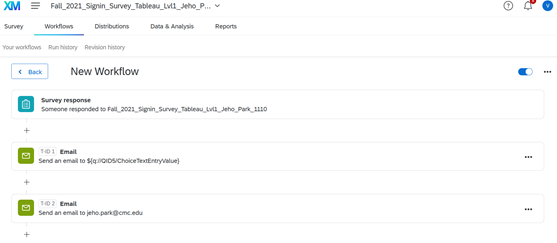
\includegraphics{https://raw.githubusercontent.com/CMC-QCL/fellow-handbook/main/Images/Qualtrics5.png?token=GHSAT0AAAAAABQHYZSFK2WX7PBTXIRZMD2CYR33C3Q}\\
    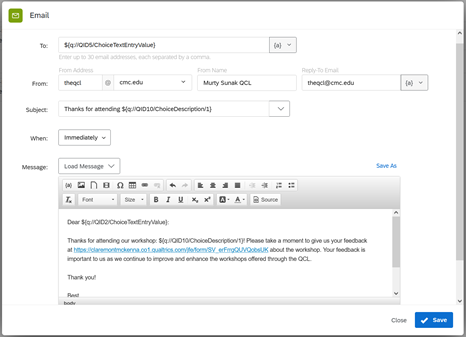
\includegraphics{https://raw.githubusercontent.com/CMC-QCL/fellow-handbook/main/Images/Qualtrics6.png?token=GHSAT0AAAAAABQHYZSEAVW7NSVB5GU2PV6KYR33C4Q}
  \end{itemize}
\end{itemize}

Step 5:

\begin{itemize}
\tightlist
\item
  Exit\\
  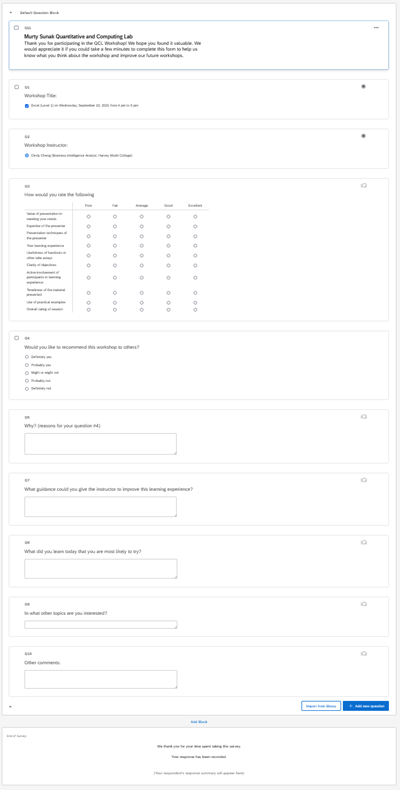
\includegraphics{https://raw.githubusercontent.com/CMC-QCL/fellow-handbook/main/Images/Qualtrics7.png?token=GHSAT0AAAAAABQHYZSFHP5BJIAYD6IUDVBSYR33C5A}
\end{itemize}

Step 6:

\begin{itemize}
\tightlist
\item
  Change workflow link

  \begin{itemize}
  \tightlist
  \item
    Make sure Dr.~Park is getting an email sent to him\\
    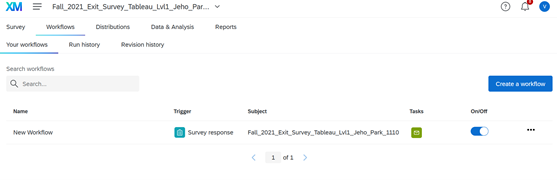
\includegraphics{https://raw.githubusercontent.com/CMC-QCL/fellow-handbook/main/Images/Qualtrics8.png?token=GHSAT0AAAAAABQHYZSFXR5CPIJLMQNPMGAUYR33C6A}
    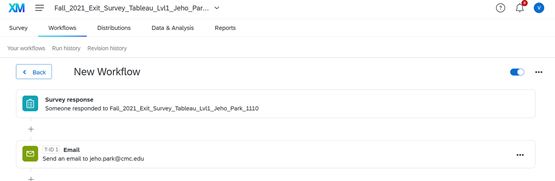
\includegraphics{https://raw.githubusercontent.com/CMC-QCL/fellow-handbook/main/Images/Qualtrics9.png?token=GHSAT0AAAAAABQHYZSE6WJWGMJCVONOBB22YR33C7A}
  \end{itemize}
\end{itemize}

Step 7:

\begin{itemize}
\tightlist
\item
  Click Publish\\
  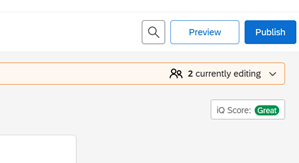
\includegraphics{https://raw.githubusercontent.com/CMC-QCL/fellow-handbook/main/Images/Qualtrics10.png?token=GHSAT0AAAAAABQHYZSEHWMYXZAQ3LAUNF64YR33C7Q}
\end{itemize}

Step 8:

\begin{itemize}
\tightlist
\item
  Copy link to use for Bit.ly later and hit publish

  \begin{itemize}
  \tightlist
  \item
    If you forget to get here, you can still get it when you make QR code\\
    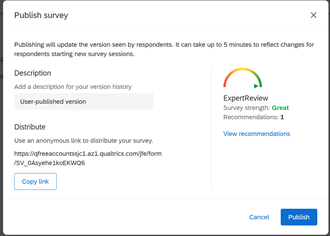
\includegraphics{https://raw.githubusercontent.com/CMC-QCL/fellow-handbook/main/Images/Qualtrics11.png?token=GHSAT0AAAAAABQHYZSFZ57JIYS3UOV2DWBGYR33DAA}
  \end{itemize}
\end{itemize}

Step 9:

\begin{itemize}
\tightlist
\item
  Barcode for Word doc

  \begin{itemize}
  \tightlist
  \item
    Anonymous link will give you the link of the survey again to put into Bit.ly\\
  \item
    Download QR code for word doc use\\
    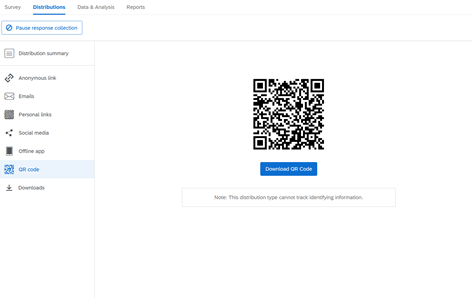
\includegraphics{https://raw.githubusercontent.com/CMC-QCL/fellow-handbook/main/Images/Qualtrics12.png?token=GHSAT0AAAAAABQHYZSE2INECCJZQNJNNUBOYR33DBA}
  \end{itemize}
\end{itemize}

\textbf{Bit.ly}

\begin{figure}
\centering
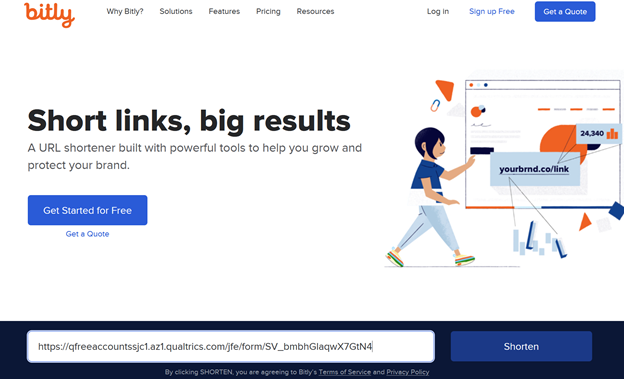
\includegraphics{https://raw.githubusercontent.com/CMC-QCL/fellow-handbook/main/Images/Bitly1.png?token=GHSAT0AAAAAABQHYZSEVUTINJ3WNDHGET6CYR34SJA}
\caption{Bit.ly}
\end{figure}

Step 1:

\begin{itemize}
\tightlist
\item
  Copy and paste the shorten link into word doc
  
\includegraphics{https://raw.githubusercontent.com/CMC-QCL/fellow-handbook/main/Images/Bitly2.png?token=GHSAT0AAAAAABQHYZSF6ATRFOGCG4O6Q5GYYR34SJQ}
\end{itemize}

Step 2:

\begin{itemize}
\tightlist
\item
  Once you create a registration form on localist, would you please create bit.ly short cut and let me know? Do you know how to create a bit.ly URL shortcut?

  \begin{itemize}
  \tightlist
  \item
    created shortcuts with some naming convention she made for herself.

    \begin{itemize}
    \tightlist
    \item
      e.g., \url{http://bit.ly/su2021-05-excel-L2-reg}
    \item
      e.g., \url{https://bit.ly/fa2021-excel-1020}
    \end{itemize}
  \end{itemize}
\end{itemize}

\textbf{Flyer Word doc}

\begin{itemize}
\tightlist
\item
  Change to fit workshop

  \begin{itemize}
  \tightlist
  \item
    Title
  \item
    Date \& Time
  \item
    Instructor
  \item
    QR Code from Qualtrics
  \item
    Shorten link from Bit.ly\\
    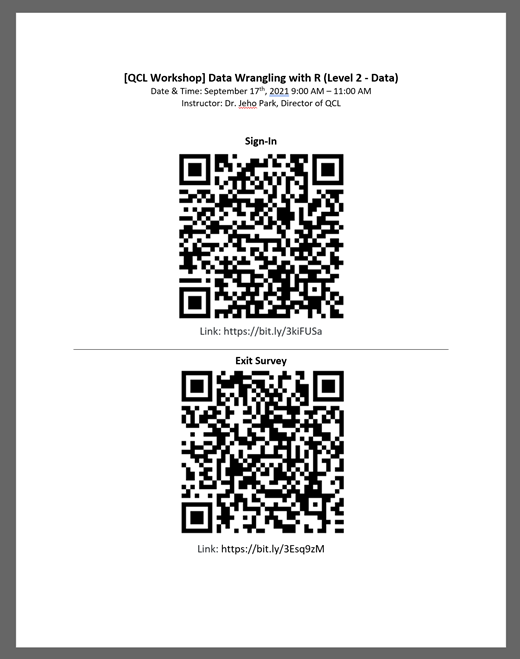
\includegraphics{https://raw.githubusercontent.com/CMC-QCL/fellow-handbook/main/Images/Flyer1.png?token=GHSAT0AAAAAABQHYZSEEVRI534IPXMIPKZQYR34TPQ}
  \end{itemize}
\end{itemize}

\textbf{Emails (to be written)}

\textbf{Reminder Email}

\begin{itemize}
\item
  Send out a reminder email.
\item
  Add

  \begin{itemize}
  \tightlist
  \item
    Virtual Work info: Zoom invitation link (just in case)
  \item
    In-Person Info:
  \item
    Anything instructor wants to relay
  \end{itemize}
\item
  Example 1\\
  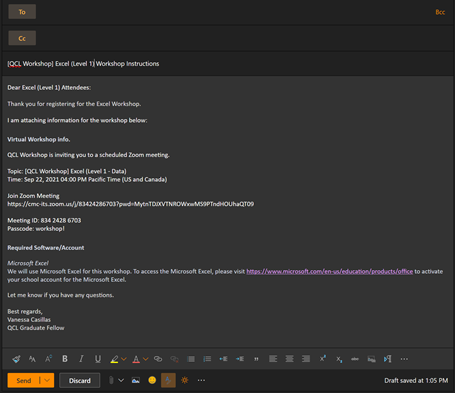
\includegraphics{https://raw.githubusercontent.com/CMC-QCL/fellow-handbook/main/Images/Reminder1.png?token=GHSAT0AAAAAABQHYZSEFV75QKPGDCD6E44WYR34UCA}
\item
  Example 2\\
  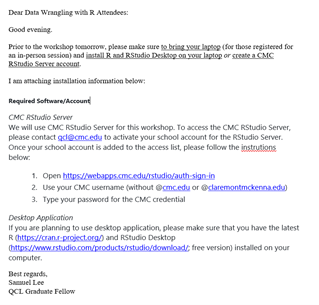
\includegraphics{https://raw.githubusercontent.com/CMC-QCL/fellow-handbook/main/Images/Reminder2.png?token=GHSAT0AAAAAABQHYZSFCTLKZSBA56T3TYOEYR34UDA}
\item
  Example 3\\
  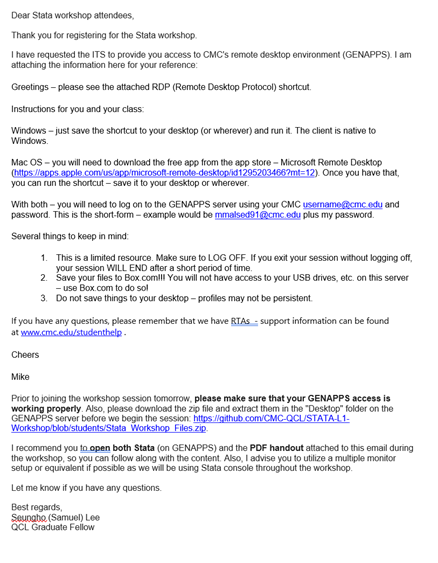
\includegraphics{https://raw.githubusercontent.com/CMC-QCL/fellow-handbook/main/Images/Reminder3.png?token=GHSAT0AAAAAABQHYZSE7YC557TFTIW6H3YEYR34UEA}
\item
  Example 4
\end{itemize}

Dear MATLAB (Level 1 -- Coding+Computing) Attendees:

Thank you for registering for the MATLAB (Level 1 -- Coding+Computing) Workshop.

Getting Equipped with MATLAB (Level 1 -- Coding+Computing)

Instructor: Bhaven Mistry (Assistant Director of the QCL)

Summary:\\
Want to learn to program, but don't know where to start or what to install? MATLAB is a numerical computing language and environment that is surprisingly easy to use. Typically used by engineers and scientists, you can think of it as a very powerful, customizable calculator. But, interestingly, it's this very characteristic that makes MATLAB an ideal language for programming beginners, even if you're not mathematically inclined.
In this workshop, we will step you through the basics of programming using the MATLAB coding environment. We will start by getting familiar with the software, learning the basics of variable assignment and manipulation, writing our own functions, and exploring some applications. If you're completely new to programming, learning the fundamentals with MATLAB first is a great way to springboard into other languages. Alternatively, if you have some experience with programming, but have always wanted to learn what MATLAB is used for, this could be a good way to get your feet wet.

Pre-requisites:\\
Internet Use: Introductory level (search, log-in, navigation of websites, etc.)
Software: Attendees are asked to have MATLAB on their computers for the workshop. MATLAB is available for CMC students and faculty at \url{https://www.cmc.edu/information-technology/academic-software}

Location:\\
Online (Attendees will receive the Zoom meeting information after registration)

Participants:

Open to all CMC Students, Faculty and Staff

I am attaching information for the workshop below:\\
QCL Workshop is inviting you to a scheduled Zoom meeting.

Topic: {[}QCL Workshop{]} Get Equipped with MATLAB

Time: Sep 29, 2021 03:00 PM Pacific Time (US and Canada)

Join Zoom Meeting

\url{https://cmc-its.zoom.us/j/83773547610?pwd=Y2loa3VoWnQvWFQxUDg1V0xIbHBNdz09}

Meeting ID: 837 7354 7610

Passcode: workshop!

Required Software/Account

\url{https://www.cmc.edu/information-technology/academic-software}

Let me know if you have any questions.

Best regards,\\
Vanessa Casillas\\
QCL Graduate Fellow

\textbf{Attendees Emails}

\begin{itemize}
\item
  Go to Localist and click on event\\
  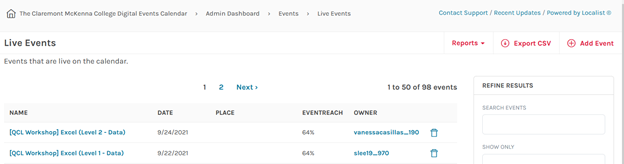
\includegraphics{https://raw.githubusercontent.com/CMC-QCL/fellow-handbook/main/Images/Attendees1.png?token=GHSAT0AAAAAABQHYZSFYHOXMYZTZYLSH53MYR34WIQ}
\item
  Click on View Confirmed Tickets\\
  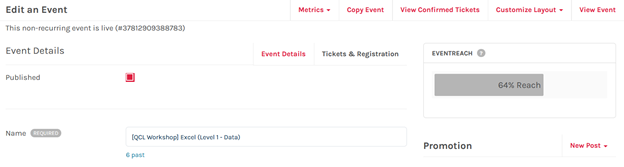
\includegraphics{https://raw.githubusercontent.com/CMC-QCL/fellow-handbook/main/Images/Attendees2.png?token=GHSAT0AAAAAABQHYZSEU4WILBVYDC2MSVJEYR34WJA}
\item
  Click Export CSV\\
  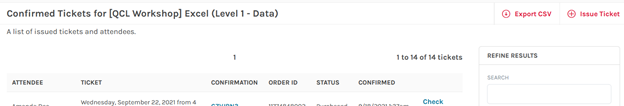
\includegraphics{https://raw.githubusercontent.com/CMC-QCL/fellow-handbook/main/Images/Attendees3.png?token=GHSAT0AAAAAABQHYZSEJHA7A4AIW3YZH2XKYR34WJA}
\item
  Go to email and download the CSV\\
  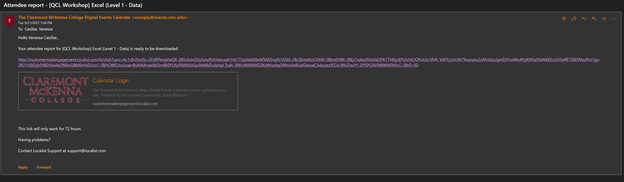
\includegraphics{https://raw.githubusercontent.com/CMC-QCL/fellow-handbook/main/Images/Attendees4.png?token=GHSAT0AAAAAABQHYZSEKGQ5RYLLDX3WBLGAYR34WJQ}
\item
  Open CSV and copy emails into your reminder email\\
  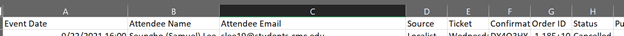
\includegraphics{https://raw.githubusercontent.com/CMC-QCL/fellow-handbook/main/Images/Attendees5.png?token=GHSAT0AAAAAABQHYZSFR7C4WRV7FXZS5XZSYR34WKQ}
\end{itemize}

\hypertarget{day-of-workshop}{%
\subsubsection{\texorpdfstring{Day of workshop }{Day of workshop }}\label{day-of-workshop}}

\textbf{Moderator checklist}

\begin{itemize}
\tightlist
\item
  Morning of

  \begin{itemize}
  \tightlist
  \item
    Paste Zoom info in QCL Workshop -- Workshop Control Booth chat in Teams
  \item
    Send out reminders if you haven't already
  \end{itemize}
\item
  Show up 30 minutes before workshop

  \begin{itemize}
  \tightlist
  \item
    Print out flyers

    \begin{itemize}
    \tightlist
    \item
      Put on tables where the attendees will sit
    \end{itemize}
  \item
    Log into Zoom (workshops)

    \begin{itemize}
    \tightlist
    \item
      Start 30 minutes before
    \item
      Check audio and video
    \item
      Make Instructor co-host
    \item
      Test runs with instructor
    \end{itemize}
  \item
    Get shorten links from bit.ly ready
  \item
    Set-up camera
  \item
    Put the spotlight on workshop video feed
  \item
    Make sure the instructor is screensharing
  \end{itemize}
\item
  Time of the workshop

  \begin{itemize}
  \tightlist
  \item
    Welcome everyone: (change when necessary for only virtual or only in person workshops)

    \begin{itemize}
    \tightlist
    \item
      Welcome to the QCL! Today's workshop is (name of event) instructed by (name of instructor. My name is (your name) and I (as well as (other moderator)) will your moderators for today's workshop. If you have any questions or concerns throughout the session, please write in chat for our virtual attendees or raise or have for our in-person attendees. Before we start, please make sure to sign in with either the QR code or the link provided. Lastly, this workshop will be recorded. Enjoy!
    \item
      Link sign-in survey in chat and links for workshop from instructor
      Welcome! Please sign-in: \url{https://bit.ly/3zDNzPj}
      Link from instructor: \url{https://github.com/CMC-QCL/Excel-L2-Workshop}
      If you have any questions or concerns throughout the session, please write in chat \citet{everyone}.
      Thank you! Please sign-out: \url{https://bit.ly/3EIOgdX}
    \end{itemize}
  \item
    Click Record

    \begin{itemize}
    \tightlist
    \item
      Note: if on break, click pause not stop, we want the least number of files made
    \end{itemize}
  \item
    Check in attendees who attend on Localist

    \begin{itemize}
    \tightlist
    \item
      Cross check over Qualtrics to make sure that attendees take survey as well
    \end{itemize}
  \item
    Interrupt the instructor if an attendee online has a question or if the attendee in-person has not been seen raising their hand.
  \end{itemize}
\item
  End of workshop

  \begin{itemize}
  \tightlist
  \item
    Link Exit survey in chat
  \item
    Thank everyone for coming
  \item
    Clean up and back up
  \end{itemize}
\item
  Send email reminder if there is a low rate for surveys
\item
  Send zoom meeting recordings to attendees that attended

  \begin{itemize}
  \tightlist
  \item
    Note: after every semester we dump recordings into a box file, before CMC does it
  \end{itemize}
\end{itemize}

\hypertarget{day-after-workshop}{%
\subsubsection{\texorpdfstring{Day after workshop }{Day after workshop }}\label{day-after-workshop}}

\textbf{Qualtrics}

\begin{itemize}
\tightlist
\item
  Give ``Collaborate'' to instructor on surveys
\end{itemize}

\textbf{Zoom Recordings}

\begin{itemize}
\tightlist
\item
  Only provided to the attendees that showed up for the workshop
\item
  Records are ready to send the next day after the workshop
  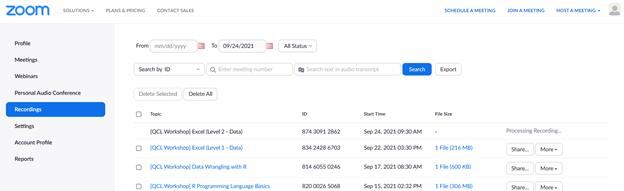
\includegraphics{https://raw.githubusercontent.com/CMC-QCL/fellow-handbook/main/Images/Zoom1.png?token=GHSAT0AAAAAABQHYZSFNEPWMMCXVFZZCKTAYR34ZEA}
\end{itemize}

\textbf{Ending email example}

Subject: Thank you for attending the (name of workshop) Workshop

Hello (name of workshop) attendees,

Thank you for attending the workshop.

I have provided the links for sign-in and sign-out:

Sign-in:
(Link of survey)

Sign-out:
(Link of survey)

Please make sure to complete the surveys, they count as your attendance. If you have already completed them, thank you.

(all pasted from zoom)

Note: records are only provided if you attend the workshop

Lastly, if there was any homework assigned for this workshop, please send all documents to: \href{mailto:qcl@cmc.edu}{\nolinkurl{qcl@cmc.edu}} for grading.

Thank you,
(your name)
QCL Graduate Fellow

\hypertarget{workshop-issues}{%
\subsubsection{\texorpdfstring{Workshop Issues }{Workshop Issues }}\label{workshop-issues}}

\textbf{New attendees after closed registration}

\begin{itemize}
\tightlist
\item
  Email to student for information: (Do not to ask for people's gender for the new attendee's emails as it is optional on our form.)
\end{itemize}

Subject: {[}QCL{]} Online Workshop on name (date at time) and name (date at time)\\
{[}Bcc'd everyone else except QCL Fellows{]}

Hi (name of new attendee),

Would you like to register for both Excel 1 and Excel 2 sessions?

Also, are you able to provide me following information?\\
1. Please enter your student ID \# (Must be 8 characters). For all faculty/staff/non-Claremont Colleges person, please insert 00000000.\\
2. Gender\\
3. Are you a Freshman, Sophomore, Junior, Senior, Graduate Student, Faculty, Staff or Other?

Please note that we usually close registration 1 to 3 days prior (depending on the preparation needed to set up a working environment) to workshop events.

Best regards,\\
QCL Graduate Fellow (put your name here)

\begin{itemize}
\item
  Issue Ticket tab on Confirmed Tickets page
  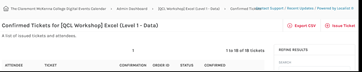
\includegraphics{https://raw.githubusercontent.com/CMC-QCL/fellow-handbook/main/Images/Issues1.png?token=GHSAT0AAAAAABQHYZSFWCJTJPCOOVZB6BMCYR3662A}
\item
  Fill in all info
  \includegraphics{https://raw.githubusercontent.com/CMC-QCL/fellow-handbook/main/Images/Issues2.png?token=GHSAT0AAAAAABQHYZSFGNXR2K3YP4MPAUKIYR3662Q}
\item
  After filling out the form, the attendee will get an email from Localist

  \begin{itemize}
  \tightlist
  \item
    Send out an email follow up to the new attendee
  \end{itemize}
\end{itemize}

Subject: {[}QCL Workshop{]} Name of workshop -- Availability

Hi (name of new attendee),

I have input your information into Localist for the (name of workshop) workshop.

You should have received a Localist ticket by now.

Please let me know if you have any questions.

Best regards,
QCL Graduate Fellow (put your name here)

\begin{itemize}
\tightlist
\item
  If you just input, the new attendee without information, send this email
\end{itemize}

Subject: {[}QCL Workshop{]} Name of workshop -- Availability

Hi (name of new attendee),

I just received a message from Janna that you would like to register for the (name of workshop) workshop.

You should have received a Localist ticket by now.

Please let me know if you have any questions.

Best regards,
QCL Graduate Fellow (put your name here)

\begin{itemize}
\tightlist
\item
  Note: We typically have 15 seats but wait list is 5
\end{itemize}

\textbf{Check attendee's emails}

\begin{itemize}
\tightlist
\item
  Fix emails, sometimes they misspell their emails
\end{itemize}

\hypertarget{e.-buying-a-ticket-making-sure-it-works}{%
\subsubsection{\texorpdfstring{e. Buying a ticket -- Making sure it works }{e. Buying a ticket -- Making sure it works }}\label{e.-buying-a-ticket-making-sure-it-works}}

pic3
\includegraphics{https://raw.githubusercontent.com/CMC-QCL/fellow-handbook/main/Images/buying1.png?token=GHSAT0AAAAAABQHYZSEAFJXIGCEG5G6GJ2YYR37A3A}\\
pic4
\includegraphics{https://raw.githubusercontent.com/CMC-QCL/fellow-handbook/main/Images/buying2.png?token=GHSAT0AAAAAABQHYZSEJ6IPZ3I33FFLKKKWYR37A4A}\\
pic5
\includegraphics{https://raw.githubusercontent.com/CMC-QCL/fellow-handbook/main/Images/buying3.png?token=GHSAT0AAAAAABQHYZSFNCRRMHYYIG6XM63SYR37A4Q}\\
pic6
\includegraphics{https://raw.githubusercontent.com/CMC-QCL/fellow-handbook/main/Images/buying4.png?token=GHSAT0AAAAAABQHYZSFR3JR4OJXIYRQOHHOYR37A4Q}\\
pic7
\includegraphics{https://raw.githubusercontent.com/CMC-QCL/fellow-handbook/main/Images/buying5.png?token=GHSAT0AAAAAABQHYZSFFCYR37LJGG5KPU76YR37A5Q}\\
pic8
\includegraphics{https://raw.githubusercontent.com/CMC-QCL/fellow-handbook/main/Images/buying6.png?token=GHSAT0AAAAAABQHYZSFC3TW45QTT24S7IEMYR37A6A}\\
pic9
\includegraphics{https://raw.githubusercontent.com/CMC-QCL/fellow-handbook/main/Images/buying7.png?token=GHSAT0AAAAAABQHYZSFJYCEZRTXOBKKSXWWYR37A7A}

\hypertarget{f.-changing-website}{%
\subsubsection{\texorpdfstring{f.~Changing Website }{f.~Changing Website }}\label{f.-changing-website}}

pic10
\includegraphics{https://raw.githubusercontent.com/CMC-QCL/fellow-handbook/main/Images/website1.png?token=GHSAT0AAAAAABQHYZSF424DMO6WYEUA6L4SYR37DLQ}
pic11
\includegraphics{https://raw.githubusercontent.com/CMC-QCL/fellow-handbook/main/Images/website2.png?token=GHSAT0AAAAAABQHYZSFDBFXWK6DHPJLR2B4YR37DMQ}
pic12
\includegraphics{https://raw.githubusercontent.com/CMC-QCL/fellow-handbook/main/Images/website3.png?token=GHSAT0AAAAAABQHYZSFHHNPWTPCECXAZXPCYR37DNQ}
pic13
\includegraphics{https://raw.githubusercontent.com/CMC-QCL/fellow-handbook/main/Images/website4.png?token=GHSAT0AAAAAABQHYZSEPS3BFP6GID2MUBQSYR37DOA}

\hypertarget{g.-checklist-for-a-typical-workday}{%
\subsubsection{\texorpdfstring{g. Checklist for a Typical Workday }{g. Checklist for a Typical Workday }}\label{g.-checklist-for-a-typical-workday}}

This is if there is no workshop or appointment going on

\begin{itemize}
\tightlist
\item
  Check email

  \begin{itemize}
  \tightlist
  \item
    Write back to anyone
  \item
    Send any emails that have been on TODO list
  \item
    Organize your emails in their respective folders
    \includegraphics{https://raw.githubusercontent.com/CMC-QCL/fellow-handbook/main/Images/Checklist1.png?token=GHSAT0AAAAAABQHYZSEWFYFXOGNZOIRQCD2YR37EVA}
  \end{itemize}
\item
  Update QCL website
\item
  Day after workshop

  \begin{itemize}
  \tightlist
  \item
    Send out email of closing workshop

    \begin{itemize}
    \tightlist
    \item
      Recording, survey links, thank you
    \end{itemize}
  \end{itemize}
\item
  Two weeks prior work

  \begin{itemize}
  \tightlist
  \item
    Check what is coming in two weeks

    \begin{itemize}
    \tightlist
    \item
      Set appointments to meet with instructors

      \begin{itemize}
      \tightlist
      \item
        Get summaries
      \item
        Tools
      \item
        Point points
      \item
        files
      \item
        Licenses
      \end{itemize}
    \end{itemize}
  \end{itemize}
\item
  One week before work

  \begin{itemize}
  \tightlist
  \item
    Localist and zoom
  \item
    Let Dr.~Park know they are ready to be announced
  \end{itemize}
\item
  Two days before work

  \begin{itemize}
  \tightlist
  \item
    Send out reminder emails to localist attendees for upcoming workshop
  \end{itemize}
\item
  Get licenses information out

  \begin{itemize}
  \tightlist
  \item
    Close old Qualtrics surveys
  \item
    Make new Qualtrics surveys for upcoming workshops
  \item
    Make QR codes/Bit.ly for upcoming workshop
    Other work
  \item
    Graphic Design
  \end{itemize}
\item
  Make workshops

  \begin{itemize}
  \tightlist
  \item
    SQL
  \item
    EXCEL
  \item
    GIS
  \end{itemize}
\item
  Workday

  \begin{itemize}
  \tightlist
  \item
    Put in schedule
  \end{itemize}
\end{itemize}

\hypertarget{h.-building-a-workshop}{%
\subsubsection{\texorpdfstring{h. Building a Workshop }{h. Building a Workshop }}\label{h.-building-a-workshop}}

\textbf{Github}

\begin{figure}
\centering
\includegraphics{https://raw.githubusercontent.com/CMC-QCL/fellow-handbook/main/Images/Building1.png?token=GHSAT0AAAAAABQHYZSEFOTOYD3FTUQAX2TUYR37FSA}
\caption{pic15}
\end{figure}

\begin{itemize}
\tightlist
\item
  Files needed in Github

  \begin{itemize}
  \tightlist
  \item
    Pre-workshop requirements
  \item
    Presentation pdf
  \item
    Files for hand-on activities
  \item
    README.md

    \begin{itemize}
    \tightlist
    \item
      A summary of the workshop for localist and zoom
    \end{itemize}
  \end{itemize}
\end{itemize}

\begin{figure}
\centering
\includegraphics{https://raw.githubusercontent.com/CMC-QCL/fellow-handbook/main/Images/Building2.png?token=GHSAT0AAAAAABQHYZSFGE7LSNWTU5HKIM36YR37FSQ}
\caption{A summary of the workshop for localist and zoom}
\end{figure}

\textbf{Pre-workshop requirements PDF}

\begin{itemize}
\tightlist
\item
  Make in program you would like to use (i.e., Powerpoint, ArcGis Stories)
\item
  Make it into a PDF to send before workshop
\item
  Downloading software How to for Mac and Windows
\item
  License information
\item
  Explain what to bring to workshop
\end{itemize}

\textbf{Presentation PDF}
* Make in program you would like to use (i.e., Powerpoint, ArcGis Stories)
- Make it into a PDF to send after workshop
- Beginners' material for Level 1
- Required Slides (make sure to do the material in chucks)
- Title page
- Before we start
- Download Information
- Agenda
- Overview
- Vocabulary
- Today's Data
- Demo Agenda
- Demo Slides
- Activity
- Questions
- Answers
- Resources
- Contact info

\textbf{Files}

\begin{itemize}
\tightlist
\item
  Data files to import

  \begin{itemize}
  \tightlist
  \item
    Hand-on activities
  \end{itemize}
\item
  Other files of interest
\end{itemize}

\hypertarget{i.-workshops-building}{%
\subsubsection{\texorpdfstring{i. Workshops Building }{i. Workshops Building }}\label{i.-workshops-building}}

\begin{itemize}
\tightlist
\item
  In the past, the way we offer our workshop to specific institute like Lowe was that we (Cindy) worked with their admin or student leader to find good times for their fellows and RAs and offer a separate workshop(s) for them. I am thinking we would want to offer them a separate GIS workshop(s).
\end{itemize}

Who asked for QCL trainings:

\href{mailto:brooke.bernal@claremontmckenna.edu}{\nolinkurl{brooke.bernal@claremontmckenna.edu}} (Rose Institute)\\
\href{mailto:brittany.bras@claremontmckenna.edu}{\nolinkurl{brittany.bras@claremontmckenna.edu}} (Rose Institute)\\
\href{mailto:Kristin.Miller@ClaremontMcKenna.edu}{\nolinkurl{Kristin.Miller@ClaremontMcKenna.edu}} (Roberts Environment Center)\\
\href{mailto:npatel21@students.claremontmckenna.edu}{\nolinkurl{npatel21@students.claremontmckenna.edu}} (Student Manager Rose Institute)\\
\href{mailto:jennifer.feitosa@claremontmckenna.edu}{\nolinkurl{jennifer.feitosa@claremontmckenna.edu}} (Psychology, asked for SPSS and Excel)

Who you can ask for QCL workshops:

Jeanine Finn \href{mailto:jeanine.finn@claremont.edu}{\nolinkurl{jeanine.finn@claremont.edu}} (Unix Shell and Git)\\
Brandon Bak \href{mailto:brandonbak@gmail.com}{\nolinkurl{brandonbak@gmail.com}} (Alteryx)\\
Cindy Cheng \href{mailto:cindy.cheng@cgu.edu}{\nolinkurl{cindy.cheng@cgu.edu}} (Power BI)\\
Alfonso Landeros \href{mailto:alanderos@ucla.edu}{\nolinkurl{alanderos@ucla.edu}} (Julia)\\
Aashita Kesarwani \href{mailto:akesarwani@hmc.edu}{\nolinkurl{akesarwani@hmc.edu}} (ML)\\
Brad McCauley \href{mailto:bmccauley@hmc.edu}{\nolinkurl{bmccauley@hmc.edu}} (bash script)

SQL dataset used for Fall 2020 attached.

\hypertarget{j.-zoom-recording-downloads}{%
\subsubsection{\texorpdfstring{j. Zoom Recording Downloads }{j. Zoom Recording Downloads }}\label{j.-zoom-recording-downloads}}

We are reaching out today with a friendly and important reminder to please transfer or delete your older Zoom cloud recordings within your Zoom account to help ensure that we can continue to provide this service to our faculty and staff without accruing additional storage expenses.

Our Zoom cloud recording storage currently has a shared quota of 1 terabyte for all users and about 1 gigabyte of storage per individual user. However, we now have several Zoom accounts that are way over the 1 gigabyte storage allotment. To collectively help save space, we recommend that all users download their Zoom recordings and store them in an alternate location, such as Box where much more storage space is available. Once you've stored the recordings in an alternate location, please make sure to go back and delete the recordings from your Zoom cloud storage.

Action Needed:

\begin{itemize}
\tightlist
\item
  If you use Zoom cloud recording -- please follow the below instructions for offloading your recordings and then delete them off Zoom once transferred
\end{itemize}

\emph{How to Download Your Zoom Cloud Recordings:}

\begin{enumerate}
\def\labelenumi{\arabic{enumi}.}
\item
  Login to the Zoom.us web portal (\url{https://zoom.us})
\item
  In the left-hand navigation menu, click Recordings (direct link: \url{https://zoom.us/recording})
\item
  Click More next to a meeting recording and click Download
\end{enumerate}

\begin{figure}
\centering
\includegraphics{https://raw.githubusercontent.com/CMC-QCL/fellow-handbook/main/Images/Recording1.png?token=GHSAT0AAAAAABQHYZSE62MPXWLO7RAVXLT2YR37G7Q}
\caption{Click More next to a meeting recording and click Download}
\end{figure}

\begin{enumerate}
\def\labelenumi{\arabic{enumi}.}
\setcounter{enumi}{3}
\tightlist
\item
  Click Download on the pop-up that appears
\end{enumerate}

\begin{figure}
\centering
\includegraphics{https://raw.githubusercontent.com/CMC-QCL/fellow-handbook/main/Images/Recording2.png?token=GHSAT0AAAAAABQHYZSEDGFDZMEIKP7HMG7SYR37HBA}
\caption{Click Download on the pop-up that appears}
\end{figure}

\begin{enumerate}
\def\labelenumi{\arabic{enumi}.}
\setcounter{enumi}{4}
\tightlist
\item
  Click Allow if prompted for permission to Download multiple files.
\end{enumerate}

\begin{figure}
\centering
\includegraphics{https://raw.githubusercontent.com/CMC-QCL/fellow-handbook/main/Images/Recording3.png?token=GHSAT0AAAAAABQHYZSEFR6W6JMYF4LAP262YR37HCA}
\caption{Click Allow if prompted for permission to Download multiple files.}
\end{figure}

\begin{enumerate}
\def\labelenumi{\arabic{enumi}.}
\setcounter{enumi}{5}
\tightlist
\item
  Check your Downloads folder for your recording files (.m4a for audio and .mp4 for video)
\end{enumerate}

Once downloaded, you can upload your files to your Box account (\url{https://claremontmckenna.box.com}). Box has a very large storage capacity per user and can be increased when necessary.

Once your files are on Box or stored somewhere safe off Zoom, you can share your files with others using the instructions outlined in the attached PDF guide called ``Sharing Files in Box''.

Alternatively, if you'd like to use local recording instead with Zoom, we have attached guides for this as well. However, we only recommend this for non-critical events and for use outside of the classroom setting.

pic20
\includegraphics{https://raw.githubusercontent.com/CMC-QCL/fellow-handbook/main/Images/Recording4.png?token=GHSAT0AAAAAABQHYZSFFBRNZCE73YNQDQA2YR37JEQ}
pic21
\includegraphics{https://raw.githubusercontent.com/CMC-QCL/fellow-handbook/main/Images/Recording5.png?token=GHSAT0AAAAAABQHYZSFFY4ZCYXKFX7QENZUYR37JEQ}
pic22
\includegraphics{https://raw.githubusercontent.com/CMC-QCL/fellow-handbook/main/Images/Recording6.png?token=GHSAT0AAAAAABQHYZSFI6NFT74NMRKJD62CYR37JFA}
pic23
\includegraphics{https://raw.githubusercontent.com/CMC-QCL/fellow-handbook/main/Images/Recording7.png?token=GHSAT0AAAAAABQHYZSEHPDCRTORT2XWDEFGYR37JGA}
pic24
\includegraphics{https://raw.githubusercontent.com/CMC-QCL/fellow-handbook/main/Images/Recording8.png?token=GHSAT0AAAAAABQHYZSE7T2RLT63GUX22AGMYR37JGQ}
pic25
\includegraphics{https://raw.githubusercontent.com/CMC-QCL/fellow-handbook/main/Images/Recording9.png?token=GHSAT0AAAAAABQHYZSE642CXKBLSFSNXCL4YR37JHA}
pic26
\includegraphics{https://raw.githubusercontent.com/CMC-QCL/fellow-handbook/main/Images/Recording10.png?token=GHSAT0AAAAAABQHYZSEJT5QOBTICOAS2IRAYR37JIA}
pic27
\includegraphics{https://raw.githubusercontent.com/CMC-QCL/fellow-handbook/main/Images/Recording11.png?token=GHSAT0AAAAAABQHYZSFQU6HR6EGUVNOGMVCYR37JIQ}

\hypertarget{k.-qualtrics-make-a-workflow}{%
\subsubsection{\texorpdfstring{k. Qualtrics Make a Workflow }{k. Qualtrics Make a Workflow }}\label{k.-qualtrics-make-a-workflow}}

\begin{itemize}
\tightlist
\item
  Sign-in Survey
\end{itemize}

qual1
\includegraphics{https://raw.githubusercontent.com/CMC-QCL/fellow-handbook/main/Images/Qual1.png?token=GHSAT0AAAAAABQHYZSFAVJYDNSGBSMCS6YIYR37RKA}
qual2
\includegraphics{https://raw.githubusercontent.com/CMC-QCL/fellow-handbook/main/Images/Qual2.png?token=GHSAT0AAAAAABQHYZSFGDKV4VYMVR2SM5Y6YR37RMA}
qual3
\includegraphics{https://raw.githubusercontent.com/CMC-QCL/fellow-handbook/main/Images/Qual3.png?token=GHSAT0AAAAAABQHYZSE6I6LWORMAWN2GJWOYR37RNA}
qual4
\includegraphics{https://raw.githubusercontent.com/CMC-QCL/fellow-handbook/main/Images/Qual4.png?token=GHSAT0AAAAAABQHYZSFH6S2YMKMD7R7TE6CYR37RNQ}
qual5
\includegraphics{https://raw.githubusercontent.com/CMC-QCL/fellow-handbook/main/Images/Qual5.png?token=GHSAT0AAAAAABQHYZSEOSFZWD7HN47ROR3SYR37ROA}
qual6
\includegraphics{https://raw.githubusercontent.com/CMC-QCL/fellow-handbook/main/Images/Qual6.png?token=GHSAT0AAAAAABQHYZSECYUJA2DVCQDGTL62YR37ROQ}
qual7
\includegraphics{https://raw.githubusercontent.com/CMC-QCL/fellow-handbook/main/Images/Qual7.png?token=GHSAT0AAAAAABQHYZSENZPEXZQ6RGXAKSOKYR37RRA}
qual8
\includegraphics{https://raw.githubusercontent.com/CMC-QCL/fellow-handbook/main/Images/Qual8.png?token=GHSAT0AAAAAABQHYZSEGHRTHBWHYCKCSM3SYR37STQ}
qual9
\includegraphics{https://raw.githubusercontent.com/CMC-QCL/fellow-handbook/main/Images/Qual9.png?token=GHSAT0AAAAAABQHYZSFL6LKT4TI3DORXQ3CYR37SUA}
qual10
\includegraphics{https://raw.githubusercontent.com/CMC-QCL/fellow-handbook/main/Images/Qual10.png?token=GHSAT0AAAAAABQHYZSEX6YQPGELBBWD7R2QYR37SVQ}
qual11
\includegraphics{https://raw.githubusercontent.com/CMC-QCL/fellow-handbook/main/Images/Qual11.png?token=GHSAT0AAAAAABQHYZSFGPJ3ZRZY6D35D3G4YR37SWA}
qual12
\includegraphics{https://raw.githubusercontent.com/CMC-QCL/fellow-handbook/main/Images/Qual12.png?token=GHSAT0AAAAAABQHYZSFQIZKLV3YF6B2RSIUYR37SWQ}
qual13
\includegraphics{https://raw.githubusercontent.com/CMC-QCL/fellow-handbook/main/Images/Qual13.png?token=GHSAT0AAAAAABQHYZSEJDJ5H6NAWWJJCFI4YR37TRQ}
qual14
\includegraphics{https://raw.githubusercontent.com/CMC-QCL/fellow-handbook/main/Images/Qual14.png?token=GHSAT0AAAAAABQHYZSETWRJIT37YLMB7FQOYR37TSA}
qual15
\includegraphics{https://raw.githubusercontent.com/CMC-QCL/fellow-handbook/main/Images/Qual15.png?token=GHSAT0AAAAAABQHYZSFOAYOQL7ZL5UWI6CKYR37TSQ}
qual16
\includegraphics{https://raw.githubusercontent.com/CMC-QCL/fellow-handbook/main/Images/Qual16.png?token=GHSAT0AAAAAABQHYZSFS4YFRNG5DCWECFOAYR37TUQ}

\begin{itemize}
\tightlist
\item
  Exit Survey
\end{itemize}

qual17
\includegraphics{https://raw.githubusercontent.com/CMC-QCL/fellow-handbook/main/Images/Qual17.png?token=GHSAT0AAAAAABQHYZSERIFTA2BPO4ABXVZQYR37UJQ}
qual18
\includegraphics{https://raw.githubusercontent.com/CMC-QCL/fellow-handbook/main/Images/Qual18.png?token=GHSAT0AAAAAABQHYZSF5CLB6LZNHZ4YXZGYYR37UKA}
qual19
\includegraphics{https://raw.githubusercontent.com/CMC-QCL/fellow-handbook/main/Images/Qual19.png?token=GHSAT0AAAAAABQHYZSFL4E6K7FRCO5XP4PCYR37UKQ}
qual20
\includegraphics{https://raw.githubusercontent.com/CMC-QCL/fellow-handbook/main/Images/Qual20.png?token=GHSAT0AAAAAABQHYZSF3KBN6HZXVRARM64IYR37ULA}
qual21
\includegraphics{https://raw.githubusercontent.com/CMC-QCL/fellow-handbook/main/Images/Qual21.png?token=GHSAT0AAAAAABQHYZSEHDMF7Y6J4GBKO4QQYR37UMA}
qual22
\includegraphics{https://raw.githubusercontent.com/CMC-QCL/fellow-handbook/main/Images/Qual22.png?token=GHSAT0AAAAAABQHYZSFLWAMHROVP6YFYIMQYR37UMA}
qual23
\includegraphics{https://raw.githubusercontent.com/CMC-QCL/fellow-handbook/main/Images/Qual23.png?token=GHSAT0AAAAAABQHYZSEVQ4DKKZBUUDVEXY2YR37WYQ}
qual24
\includegraphics{https://raw.githubusercontent.com/CMC-QCL/fellow-handbook/main/Images/Qual24.png?token=GHSAT0AAAAAABQHYZSF5NJIAMA7NFALHJQAYR37WZA}
qual25
\includegraphics{https://raw.githubusercontent.com/CMC-QCL/fellow-handbook/main/Images/Qual25.png?token=GHSAT0AAAAAABQHYZSEZYAOVKZT6DVKWUOOYR37WZQ}
qual26
\includegraphics{https://raw.githubusercontent.com/CMC-QCL/fellow-handbook/main/Images/Qual26.png?token=GHSAT0AAAAAABQHYZSF52YAWWEUC23ZB5WWYR37W2A}
qual27
\includegraphics{https://raw.githubusercontent.com/CMC-QCL/fellow-handbook/main/Images/Qual27.png?token=GHSAT0AAAAAABQHYZSEB7EOJKQN5I62PZTSYR37W2Q}
qual28
\includegraphics{https://raw.githubusercontent.com/CMC-QCL/fellow-handbook/main/Images/Qual28.png?token=GHSAT0AAAAAABQHYZSFK7ZHFMPAOKXIAA2EYR37W3A}

\begin{center}\rule{0.5\linewidth}{0.5pt}\end{center}

\hypertarget{l.-how-to-schedule-meetings-on-zoom}{%
\subsubsection{\texorpdfstring{l. How to schedule meetings on Zoom }{l. How to schedule meetings on Zoom }}\label{l.-how-to-schedule-meetings-on-zoom}}

meeting1
\includegraphics{https://raw.githubusercontent.com/CMC-QCL/fellow-handbook/main/Images/meeting1.png?token=GHSAT0AAAAAABQHYZSE24L6RMFSN4G7AUOOYR37YIA}

meeting2
\includegraphics{https://raw.githubusercontent.com/CMC-QCL/fellow-handbook/main/Images/meeting2.png?token=GHSAT0AAAAAABQHYZSEVVZOCJ4HNPKM7HWMYR37YJA}

\hypertarget{qcl-impact-report}{%
\chapter{QCL Impact Report}\label{qcl-impact-report}}

impact1
\includegraphics{https://raw.githubusercontent.com/CMC-QCL/fellow-handbook/main/Images/Impact1.png?token=GHSAT0AAAAAABQHYZSEVEU3G53QQ3BZQXQQYR37Y5A}

\begin{center}\rule{0.5\linewidth}{0.5pt}\end{center}

\hypertarget{a.-qualtrics-reports}{%
\subsubsection{\texorpdfstring{a. Qualtrics -- Reports }{a. Qualtrics -- Reports }}\label{a.-qualtrics-reports}}

ReportsQ1
\includegraphics{https://raw.githubusercontent.com/CMC-QCL/fellow-handbook/main/Images/Reportsq1.png?token=GHSAT0AAAAAABQHYZSEK6DVIFJSRAILBOAMYR3756A}
ReportsQ2
\includegraphics{https://raw.githubusercontent.com/CMC-QCL/fellow-handbook/main/Images/Reportsq2.png?token=GHSAT0AAAAAABQHYZSEQIMQXWS4SVNBR3YMYR3756Q}
ReportsQ3
\includegraphics{https://raw.githubusercontent.com/CMC-QCL/fellow-handbook/main/Images/Reportsq3.png?token=GHSAT0AAAAAABQHYZSELOCYC2CBAQYLGPB6YR3756Q}
ReportsQ4
\includegraphics{https://raw.githubusercontent.com/CMC-QCL/fellow-handbook/main/Images/Reportsq4.png?token=GHSAT0AAAAAABQHYZSFQYAO4RUT5TRQBCIQYR3757A}
ReportsQ5
\includegraphics{https://raw.githubusercontent.com/CMC-QCL/fellow-handbook/main/Images/Reportsq5.png?token=GHSAT0AAAAAABQHYZSFPPTHMNFLC2VBJZKQYR3757Q}
ReportsQ6
\includegraphics{https://raw.githubusercontent.com/CMC-QCL/fellow-handbook/main/Images/Reportsq6.png?token=GHSAT0AAAAAABQHYZSEL24FPSHNW4FYIKIUYR376AA}
ReportsQ7
\includegraphics{https://raw.githubusercontent.com/CMC-QCL/fellow-handbook/main/Images/Reportsq7.png?token=GHSAT0AAAAAABQHYZSE5FN3NJFYCCFSU2OYYR376AQ}
ReportsQ8
\includegraphics{https://raw.githubusercontent.com/CMC-QCL/fellow-handbook/main/Images/Reportsq8.png?token=GHSAT0AAAAAABQHYZSFRGGVBCQ7LWENG4PQYR376BA}
ReportsQ9
\includegraphics{https://raw.githubusercontent.com/CMC-QCL/fellow-handbook/main/Images/Reportsq9.png?token=GHSAT0AAAAAABQHYZSFVO4P7ADUHB6QWGE2YR376BQ}

\hypertarget{b.-localist-reports}{%
\subsubsection{\texorpdfstring{b. Localist -- Reports }{b. Localist -- Reports }}\label{b.-localist-reports}}

ReportsL1
\includegraphics{https://raw.githubusercontent.com/CMC-QCL/fellow-handbook/main/Images/Reportsl1.png?token=GHSAT0AAAAAABQHYZSE2XYALVHHPH6Q6HQGYR377YQ}
ReportsL2
\includegraphics{https://raw.githubusercontent.com/CMC-QCL/fellow-handbook/main/Images/Reportsl2.png?token=GHSAT0AAAAAABQHYZSFEMHNJPHV6AQ3HNL6YR377ZA}
ReportsL3
\includegraphics{https://raw.githubusercontent.com/CMC-QCL/fellow-handbook/main/Images/Reportsl3.png?token=GHSAT0AAAAAABQHYZSEZB2SIULIDRLJWZEOYR377ZQ}
ReportsL4
\includegraphics{https://raw.githubusercontent.com/CMC-QCL/fellow-handbook/main/Images/Reportsl4.png?token=GHSAT0AAAAAABQHYZSEJBDSM76BTCH5VI6SYR3772A}
ReportsL5
\includegraphics{https://raw.githubusercontent.com/CMC-QCL/fellow-handbook/main/Images/Reportsl5.png?token=GHSAT0AAAAAABQHYZSFOOEHYMKUCPQIEU3YYR3772Q}
ReportsL6
\includegraphics{https://raw.githubusercontent.com/CMC-QCL/fellow-handbook/main/Images/Reportsl6.png?token=GHSAT0AAAAAABQHYZSFKSVXZ76WZA6YZ7SSYR3773A}
ReportsL7
\includegraphics{https://raw.githubusercontent.com/CMC-QCL/fellow-handbook/main/Images/Reportsl7.png?token=GHSAT0AAAAAABQHYZSFVLA4NY3QFSE6FMJ2YR3773Q}
ReportsL8
\includegraphics{https://raw.githubusercontent.com/CMC-QCL/fellow-handbook/main/Images/Reportsl8.png?token=GHSAT0AAAAAABQHYZSE2A63PDIJIXTE5RFCYR3774A}

\hypertarget{c.-summaries}{%
\subsubsection{\texorpdfstring{c.~Summaries }{c.~Summaries }}\label{c.-summaries}}

summaries1
\includegraphics{https://raw.githubusercontent.com/CMC-QCL/fellow-handbook/main/Images/Summaries1.png?token=GHSAT0AAAAAABQHYZSEVMXGEE3IYWDWBB5YYR4ABNA}

\textbf{Missing Data}
missing1
\includegraphics{https://raw.githubusercontent.com/CMC-QCL/fellow-handbook/main/Images/Missing1.png?token=GHSAT0AAAAAABQHYZSFBMZXL6AES6XYE7XWYR4AB2A}

\textbf{Localist}
SumL1
\includegraphics{https://raw.githubusercontent.com/CMC-QCL/fellow-handbook/main/Images/Suml1.png?token=GHSAT0AAAAAABQHYZSF6TS4FM5A7J5YTMPIYR4ACAQ}

\begin{itemize}
\tightlist
\item
  Need to get Event Name and Event ID from site and manually input it in
  sumL2
  \includegraphics{https://raw.githubusercontent.com/CMC-QCL/fellow-handbook/main/Images/Suml2.png?token=GHSAT0AAAAAABQHYZSEKFK6PPPC2U4QHFC2YR4ACBA}
\end{itemize}

\textbf{Qualtrics}
sumQ1
\includegraphics{https://raw.githubusercontent.com/CMC-QCL/fellow-handbook/main/Images/Sumq1.png?token=GHSAT0AAAAAABQHYZSFLA6P47ULTCRDZAWAYR4ADBA}

\emph{Exit}
sumq2
\includegraphics{https://raw.githubusercontent.com/CMC-QCL/fellow-handbook/main/Images/Sumq2.png?token=GHSAT0AAAAAABQHYZSESMUCYRUOLBBYXX7GYR4ADBA}
sumq3
\includegraphics{https://raw.githubusercontent.com/CMC-QCL/fellow-handbook/main/Images/Sumq3.png?token=GHSAT0AAAAAABQHYZSFZNAIPJJXQD2VD7KIYR4ADBQ}

\emph{Sign in}
sumq4
\includegraphics{https://raw.githubusercontent.com/CMC-QCL/fellow-handbook/main/Images/Sumq4.png?token=GHSAT0AAAAAABQHYZSFRALSYK6NWABDNA5YYR4ADCA}
sumq5
\includegraphics{https://raw.githubusercontent.com/CMC-QCL/fellow-handbook/main/Images/Sumq5.png?token=GHSAT0AAAAAABQHYZSFIZOKNIGJC6Q5BU3AYR4ADCQ}

\hypertarget{d.-rough-draft-impact-report}{%
\subsubsection{\texorpdfstring{d.~Rough Draft Impact Report }{d.~Rough Draft Impact Report }}\label{d.-rough-draft-impact-report}}

Rough1
\includegraphics{https://raw.githubusercontent.com/CMC-QCL/fellow-handbook/main/Images/Rough1.png?token=GHSAT0AAAAAABQHYZSEC4CUOYRAPV7JNCWAYR4AEGA}
Rough2
\includegraphics{https://raw.githubusercontent.com/CMC-QCL/fellow-handbook/main/Images/Rough2.png?token=GHSAT0AAAAAABQHYZSFU2C6HPKGMXSTYYWMYR4AEGQ}
Rough3
\includegraphics{https://raw.githubusercontent.com/CMC-QCL/fellow-handbook/main/Images/Rough3.png?token=GHSAT0AAAAAABQHYZSFUOYHDTPB6ONAYPQMYR4AEHA}
Rough4
\includegraphics{https://raw.githubusercontent.com/CMC-QCL/fellow-handbook/main/Images/Rough4.png?token=GHSAT0AAAAAABQHYZSERJMKFQUSMSY2B3VWYR4AEIA}
Rough5
\includegraphics{https://raw.githubusercontent.com/CMC-QCL/fellow-handbook/main/Images/Rough5.png?token=GHSAT0AAAAAABQHYZSFZ57SJRUBJXOVQUIIYR4AEIA}

  \bibliography{book.bib,packages.bib}

\end{document}
